% Options for packages loaded elsewhere
\PassOptionsToPackage{unicode}{hyperref}
\PassOptionsToPackage{hyphens}{url}
\PassOptionsToPackage{dvipsnames,svgnames,x11names}{xcolor}
%
\documentclass[
  10pt,
]{article}
\usepackage{amsmath,amssymb}
\usepackage{iftex}
\ifPDFTeX
  \usepackage[T1]{fontenc}
  \usepackage[utf8]{inputenc}
  \usepackage{textcomp} % provide euro and other symbols
\else % if luatex or xetex
  \usepackage{unicode-math} % this also loads fontspec
  \defaultfontfeatures{Scale=MatchLowercase}
  \defaultfontfeatures[\rmfamily]{Ligatures=TeX,Scale=1}
\fi
\usepackage{lmodern}
\ifPDFTeX\else
  % xetex/luatex font selection
  \setmainfont[]{DejaVu Serif}
  \setsansfont[]{DejaVu Sans}
  \setmonofont[]{DejaVu Sans Mono}
  \setmathfont[]{Latin Modern Math}
\fi
% Use upquote if available, for straight quotes in verbatim environments
\IfFileExists{upquote.sty}{\usepackage{upquote}}{}
\IfFileExists{microtype.sty}{% use microtype if available
  \usepackage[]{microtype}
  \UseMicrotypeSet[protrusion]{basicmath} % disable protrusion for tt fonts
}{}
\makeatletter
\@ifundefined{KOMAClassName}{% if non-KOMA class
  \IfFileExists{parskip.sty}{%
    \usepackage{parskip}
  }{% else
    \setlength{\parindent}{0pt}
    \setlength{\parskip}{6pt plus 2pt minus 1pt}}
}{% if KOMA class
  \KOMAoptions{parskip=half}}
\makeatother
\usepackage{xcolor}
\usepackage[margin=2.0cm]{geometry}
\usepackage{color}
\usepackage{fancyvrb}
\newcommand{\VerbBar}{|}
\newcommand{\VERB}{\Verb[commandchars=\\\{\}]}
\DefineVerbatimEnvironment{Highlighting}{Verbatim}{commandchars=\\\{\}}
% Add ',fontsize=\small' for more characters per line
\newenvironment{Shaded}{}{}
\newcommand{\AlertTok}[1]{\textcolor[rgb]{1.00,0.00,0.00}{\textbf{#1}}}
\newcommand{\AnnotationTok}[1]{\textcolor[rgb]{0.38,0.63,0.69}{\textbf{\textit{#1}}}}
\newcommand{\AttributeTok}[1]{\textcolor[rgb]{0.49,0.56,0.16}{#1}}
\newcommand{\BaseNTok}[1]{\textcolor[rgb]{0.25,0.63,0.44}{#1}}
\newcommand{\BuiltInTok}[1]{\textcolor[rgb]{0.00,0.50,0.00}{#1}}
\newcommand{\CharTok}[1]{\textcolor[rgb]{0.25,0.44,0.63}{#1}}
\newcommand{\CommentTok}[1]{\textcolor[rgb]{0.38,0.63,0.69}{\textit{#1}}}
\newcommand{\CommentVarTok}[1]{\textcolor[rgb]{0.38,0.63,0.69}{\textbf{\textit{#1}}}}
\newcommand{\ConstantTok}[1]{\textcolor[rgb]{0.53,0.00,0.00}{#1}}
\newcommand{\ControlFlowTok}[1]{\textcolor[rgb]{0.00,0.44,0.13}{\textbf{#1}}}
\newcommand{\DataTypeTok}[1]{\textcolor[rgb]{0.56,0.13,0.00}{#1}}
\newcommand{\DecValTok}[1]{\textcolor[rgb]{0.25,0.63,0.44}{#1}}
\newcommand{\DocumentationTok}[1]{\textcolor[rgb]{0.73,0.13,0.13}{\textit{#1}}}
\newcommand{\ErrorTok}[1]{\textcolor[rgb]{1.00,0.00,0.00}{\textbf{#1}}}
\newcommand{\ExtensionTok}[1]{#1}
\newcommand{\FloatTok}[1]{\textcolor[rgb]{0.25,0.63,0.44}{#1}}
\newcommand{\FunctionTok}[1]{\textcolor[rgb]{0.02,0.16,0.49}{#1}}
\newcommand{\ImportTok}[1]{\textcolor[rgb]{0.00,0.50,0.00}{\textbf{#1}}}
\newcommand{\InformationTok}[1]{\textcolor[rgb]{0.38,0.63,0.69}{\textbf{\textit{#1}}}}
\newcommand{\KeywordTok}[1]{\textcolor[rgb]{0.00,0.44,0.13}{\textbf{#1}}}
\newcommand{\NormalTok}[1]{#1}
\newcommand{\OperatorTok}[1]{\textcolor[rgb]{0.40,0.40,0.40}{#1}}
\newcommand{\OtherTok}[1]{\textcolor[rgb]{0.00,0.44,0.13}{#1}}
\newcommand{\PreprocessorTok}[1]{\textcolor[rgb]{0.74,0.48,0.00}{#1}}
\newcommand{\RegionMarkerTok}[1]{#1}
\newcommand{\SpecialCharTok}[1]{\textcolor[rgb]{0.25,0.44,0.63}{#1}}
\newcommand{\SpecialStringTok}[1]{\textcolor[rgb]{0.73,0.40,0.53}{#1}}
\newcommand{\StringTok}[1]{\textcolor[rgb]{0.25,0.44,0.63}{#1}}
\newcommand{\VariableTok}[1]{\textcolor[rgb]{0.10,0.09,0.49}{#1}}
\newcommand{\VerbatimStringTok}[1]{\textcolor[rgb]{0.25,0.44,0.63}{#1}}
\newcommand{\WarningTok}[1]{\textcolor[rgb]{0.38,0.63,0.69}{\textbf{\textit{#1}}}}
\usepackage{longtable,booktabs,array}
\usepackage{calc} % for calculating minipage widths
% Correct order of tables after \paragraph or \subparagraph
\usepackage{etoolbox}
\makeatletter
\patchcmd\longtable{\par}{\if@noskipsec\mbox{}\fi\par}{}{}
\makeatother
% Allow footnotes in longtable head/foot
\IfFileExists{footnotehyper.sty}{\usepackage{footnotehyper}}{\usepackage{footnote}}
\makesavenoteenv{longtable}
\usepackage{graphicx}
\makeatletter
\def\maxwidth{\ifdim\Gin@nat@width>\linewidth\linewidth\else\Gin@nat@width\fi}
\def\maxheight{\ifdim\Gin@nat@height>\textheight\textheight\else\Gin@nat@height\fi}
\makeatother
% Scale images if necessary, so that they will not overflow the page
% margins by default, and it is still possible to overwrite the defaults
% using explicit options in \includegraphics[width, height, ...]{}
\setkeys{Gin}{width=\maxwidth,height=\maxheight,keepaspectratio}
% Set default figure placement to htbp
\makeatletter
\def\fps@figure{htbp}
\makeatother
\setlength{\emergencystretch}{3em} % prevent overfull lines
\providecommand{\tightlist}{%
  \setlength{\itemsep}{0pt}\setlength{\parskip}{0pt}}
\setcounter{secnumdepth}{-\maxdimen} % remove section numbering
% doc_header.tex -- LaTeX preamble additions used by build_docs.sh for every
% Markdown -> LaTeX -> PDF conversion (the documents of the folder Revision_SM_Higgs).
\usepackage{etoolbox}
% longtable may not be loaded by pandoc when a document has no table
\usepackage{longtable}
% bold vectors: \bm -> \symbf under unicode-math (XeLaTeX), bm package otherwise
\makeatletter
\@ifpackageloaded{unicode-math}{\providecommand{\bm}[1]{\symbf{#1}}}{\usepackage{bm}}
\makeatother
% smaller type in long tables so that wide audit tables fit the text width;
% inside a table a line break is allowed after an underscore of plain text
% (pandoc writes it as \_), so that long identifiers wrap inside their column
% rows are set a little apart, so that symbols with indices do not touch
\AtBeginEnvironment{longtable}{\footnotesize\renewcommand{\arraystretch}{1.45}%
  \let\sptunderscore\_\def\_{\sptunderscore\allowbreak}}
\setlength{\LTcapwidth}{\textwidth}
% A short table is kept on one page.  The build (code/scripts/keep_tables.py) ends the rows of such a table with \\*,
% which forbids a page break after a row, and sets \sptkeptpenalty to 10000 in front of the table.  This penalty is
% put here in the place of the breakpoint (penalty 0) that longtable leaves after every table, so that the paragraph
% that follows a kept table, its caption, begins on the same page; it is set back to 0 after the table.
\newcount\sptkeptpenalty
\sptkeptpenalty=0
\makeatletter
\patchcmd{\endlongtable}{\endgraf\penalty\z@\addvspace\LTpost}%
  {\endgraf\penalty\sptkeptpenalty\addvspace\LTpost\global\sptkeptpenalty=\z@}%
  {}{\PackageError{doc_header}{the end of longtable could not be patched}{The tables can still be typeset, but a short table may be separated from its caption.}}
\makeatother
% allow line breaks after slashes and hyphens inside table cells
\usepackage{xurl}
% code blocks: break over-long lines instead of running into the margin.
% Plain ``` blocks are typeset by pandoc as {verbatim}, highlighted ones
% (```bash) as {Highlighting}; both are re-declared as breakable fancyvrb
% environments.  The continuation line is marked with a small hooked arrow.
\usepackage{fvextra}
\RecustomVerbatimEnvironment{verbatim}{Verbatim}{breaklines,breakanywhere,fontsize=\small}
\makeatletter
\@ifundefined{Highlighting}{}{%
  \RecustomVerbatimEnvironment{Highlighting}{Verbatim}{breaklines,breakanywhere,fontsize=\small,commandchars=\\\{\}}}
\makeatother
% inline code (pandoc writes it as \texttt{...}): never hyphenate -- an inserted
% hyphen could be read as part of a file name -- but allow a line break after
% an underscore, slash, comma, colon or equals sign, so that long paths and
% column lists wrap inside the text width and inside table columns.
% Inside a formula (e.g. the name of a notebook symbol in an equation) the same
% command must first leave math mode, which \text of amsmath does.
\ExplSyntaxOn
\tl_new:N \l__spt_code_tl
\cs_new_protected:Npn \__spt_texttt:n #1
  {
    \tl_set:Nn \l__spt_code_tl {#1}
    \regex_replace_all:nnN { ([\/\,\:\=]) } { \1 \c{allowbreak} } \l__spt_code_tl
    \regex_replace_all:nnN { \c{_} } { \c{_} \c{allowbreak} } \l__spt_code_tl
    \group_begin: \ttfamily \hyphenchar \font = -1 \scan_stop: \l__spt_code_tl \group_end:
  }
\RenewDocumentCommand \texttt { m }
  {
    \mode_if_math:TF { \text { \__spt_texttt:n {#1} } } { \__spt_texttt:n {#1} }
  }
\ExplSyntaxOff
% A figure is written in the Markdown source as an image paragraph followed by
% a caption paragraph ("**Figure S1.** ..."), so that the caption is also
% visible on GitHub.  An image that starts a paragraph is centered.
\usepackage{graphicx}% pandoc loads it only for documents that contain an image
\NewCommandCopy\sptincludegraphics\includegraphics
\RenewDocumentCommand\includegraphics{O{} m}{%
  \ifvmode\begin{center}\sptincludegraphics[#1]{#2}\end{center}%
  \else\sptincludegraphics[#1]{#2}\fi}
% keep figures where they are referenced
\usepackage{float}
\floatplacement{figure}{H}
% running header with the document title
\usepackage{fancyhdr}
\pagestyle{fancy}
\fancyhf{}
\fancyhead[L]{\small PROJECT spacetimes, Revision\_SM\_Higgs}
\fancyhead[R]{\small\thepage}
\renewcommand{\headrulewidth}{0.4pt}
% 16x16 matrices: tighter columns so that a full matrix fits the text width
\setlength{\arraycolsep}{3.2pt}
% The documents of this project contain long tagged symbols, file paths and
% identifiers that cannot be hyphenated.  A paragraph is therefore allowed to
% have looser lines before TeX gives up and lets a line stick out of the margin.
\AtBeginDocument{\tolerance=2000 \emergencystretch=5em \hbadness=2000}
\ifLuaTeX
  \usepackage{selnolig}  % disable illegal ligatures
\fi
\IfFileExists{bookmark.sty}{\usepackage{bookmark}}{\usepackage{hyperref}}
\IfFileExists{xurl.sty}{\usepackage{xurl}}{} % add URL line breaks if available
\urlstyle{same}
\hypersetup{
  pdftitle={The dynamics in time of the Higgs superfluid},
  pdfauthor={Prepared for Patrick Lee Nash, Ph.D.},
  colorlinks=true,
  linkcolor={blue},
  filecolor={Maroon},
  citecolor={blue},
  urlcolor={blue},
  pdfcreator={LaTeX via pandoc}}

\title{The dynamics in time of the Higgs superfluid}
\usepackage{etoolbox}
\makeatletter
\providecommand{\subtitle}[1]{% add subtitle to \maketitle
  \apptocmd{\@title}{\par {\large #1 \par}}{}{}
}
\makeatother
\subtitle{Stage 6 of the revision of the hypotheses, part one, second
version, folder Revision\_SM\_Higgs of PROJECT spacetimes}
\author{Prepared for Patrick Lee Nash, Ph.D.}
\date{November 22, 2026}

\begin{document}
\maketitle

\hypertarget{what-this-document-is-and-what-it-finds}{%
\section{0. What this document is and what it
finds}\label{what-this-document-is-and-what-it-finds}}

The author asked that the hypotheses of PROJECT spacetimes be modified
so that the superfluid can be the Higgs field of the Standard Model,
with the quantum numbers of the Higgs doublet. In the second version of
the revised hypotheses, stated in Section 1, the superfluid is a
condensate of pairs of a particle of the isodoublet \(\Psi_{\rm LL}\)
with a particle of one of the two singlets \(\chi_{\rm SH}\) and
\(\chi'_{\rm SH}\). Stage 3 computed its ground state in five mean-field
methods, and stage 4 its effective potential, the masses of the gauge
bosons and its amplitude mode, the candidate for the Higgs boson. Stage
4 found the frequency of the amplitude mode from the linear response at
a frequency, in the two methods in which only the pairing terms act on
the ground state. This document is the first part of stage 6: it follows
the superfluid in time. Every method gives an equation of motion for the
state, the time-dependent mean field. A small displacement of the pair
fields from the ground state then oscillates at the frequencies of the
modes. The first version of the hypotheses (one singlet) is computed
alongside as the comparison. All quantities are in units of the momentum
cutoff \(\Lambda_{\rm LL}=1\); times are in units of
\(1/\Lambda_{\rm LL}\).

The findings:

\begin{enumerate}
\def\labelenumi{\arabic{enumi}.}
\tightlist
\item
  \textbf{The equations conserve what they must.} In all 21 runs the
  energy per volume, the charge densities of the symmetries and the
  orthonormality of the quasi-particle vectors are conserved to the
  accuracy of the integration (Section 3). The ground state stays at
  rest to \(4\times10^{-9}\).
\item
  \textbf{The time domain confirms stage 4.} In the pairing-only methods
  HS (0, 1) and HS (0, 0) a small displacement along the vacuum
  direction oscillates at \(d^0_{\rm SH}\), the frequency of the
  amplitude mode that stage 4 found, to \(2\times10^{-6}\), in both
  versions, without damping. A displacement along the custodial triplet
  oscillates at the same frequency, to \(2\times10^{-8}\) (Section 4).
  In HS (0, 0) the whole dynamics is that of Anderson pseudospins, one
  for the particles and one for the antiparticles at every momentum, to
  \(7\times10^{-9}\) (Section 2.4).
\item
  \textbf{The methods with normal self-energies.} Stage 4 did not
  compute the amplitude mode in HS (1, 1), KS and CJT. In the time
  domain, in the second version, the mode of HS (1, 1) lies at 0.810871,
  0.9736 times its \(d^0_{\rm SH}\) and below the energy 0.853584 that
  breaks a pair; it is undamped. In KS and CJT the spectrum peaks at
  0.873546, above the energy 0.768402 that breaks a pair, and the peak
  is 1.8 times wider than that of an undamped oscillation: there the
  amplitude mode decays into pairs of quasi-particles (Section 4).
\item
  \textbf{The scalar and vector terms split the triplet from the
  singlet.} In HS (1, 1) the custodial triplet oscillates at 0.828525,
  2.2 per cent above the singlet; in KS and CJT its peak lies at
  0.868711 (-0.55 per cent from the singlet). The degeneracy of stage 4
  is a property of the pairing-only methods (Section 4).
\item
  \textbf{The Josephson relation.} With a chemical potential \(\mu\) of
  the particle number, the phase of the pair fields turns at the rate
  \(2\mu\), to \(2\times10^{-9}\), while their length stays at
  \(d^0_{\rm SH}\) (Section 5).
\item
  \textbf{A large displacement.} A displacement by 0.3 of
  \(d^0_{\rm SH}\) in HS (0, 0) oscillates at 0.778887, 0.9582 times
  \(d^0_{\rm SH}\): the oscillation softens with its amplitude, as on a
  Mexican hat (Section 5).
\item
  \textbf{KS and CJT} give the same dynamics, to \(5\times10^{-8}\)
  (Section 3), as they gave the same ground states and susceptibilities.
\end{enumerate}

``I'' in this document is the assistant that does the work.

\hypertarget{the-hypotheses-and-the-ground-state}{%
\section{1. The hypotheses and the ground
state}\label{the-hypotheses-and-the-ground-state}}

\hypertarget{the-fields-and-their-charges}{%
\subsection{1.1 The fields and their
charges}\label{the-fields-and-their-charges}}

There are three spinor fields, all four-component Dirac fields of
\(SL(2,\mathbb C)\) and all singlets of colour:

\begin{itemize}
\tightlist
\item
  the isodoublet \(\Psi_{\rm LL}\) has eight components, numbered
  \(2d+s\), where \(d=0,\dots,3\) is the Dirac index of the chiral basis
  and \(s=0\) (up) or \(s=1\) (down) is the isospin index;
\item
  the singlets \(\chi_{\rm SH}\) and \(\chi'_{\rm SH}\) have four
  components each, numbered by the Dirac index.
\end{itemize}

The masses are
\(m_{\rm LL}=m^\chi_{\rm SH}=m^{\chi'}_{\rm SH}=0.2\,\Lambda_{\rm LL}\).
Together the three fields form one field of sixteen components,
\(\Psi_{\rm SH}=(\Psi_{\rm LL},\chi_{\rm SH},\chi'_{\rm SH})\):
components 0 to 7 are those of \(\Psi_{\rm LL}\), 8 to 11 those of
\(\chi_{\rm SH}\) and 12 to 15 those of \(\chi'_{\rm SH}\).

The gauge group is \(SL(2,\mathbb C)\times SU(2)_L\times U(1)_Y\). The
generators \(T^{a,{\rm SM}}\) (\(a=1,2,3\)) of \(SU(2)_L\) act as
\(\mathsf 1_4\otimes\tfrac12\tau^a\) on \(\Psi_{\rm LL}\) and as 0 on
the singlets, where \(\tau^a\) are the Pauli matrices. The hypercharge
\(Y^{\rm SM}\) is \(\tfrac14\) on \(\Psi_{\rm LL}\) and
\(\chi_{\rm SH}\) and \(-\tfrac34\) on \(\chi'_{\rm SH}\), and the
electric charge is \(Q^{\rm SM}=T^{3,{\rm SM}}+Y^{\rm SM}\). Two further
numbers are conserved, global symmetries that are not gauged:

\begin{itemize}
\tightlist
\item
  the particle number \(F^{\rm tot}_{\rm SH}\), 1 on every component;
\item
  the relative number \(R_{\rm SH}\), \(+1\) on the components of
  \(\Psi_{\rm LL}\) and \(-1\) on those of the singlets.
\end{itemize}

With equal masses there is one more symmetry, the custodial group
\(SU(2)_{\rm R}\). Its generators \(T^{a,{\rm R}}_{\rm SH}\) act as
\(\tfrac12\tau^a\) on the pair of singlets
\((\chi_{\rm SH},\chi'_{\rm SH})\), taken as a doublet with
\(\chi_{\rm SH}\) above, and as 0 on \(\Psi_{\rm LL}\). The hypercharge
is the combination
\(Y^{\rm SM}=T^{3,{\rm R}}_{\rm SH}+\tfrac14R_{\rm SH}\). The eight
generators \(T^{a,{\rm SM}}\), \(T^{a,{\rm R}}_{\rm SH}\),
\(R_{\rm SH}\) and \(F^{\rm tot}_{\rm SH}\) form the global group of the
hypotheses.

\sptkeptpenalty=10000
\begin{longtable}[]{@{}
  >{\raggedright\arraybackslash}p{(\columnwidth - 12\tabcolsep) * \real{0.1429}}
  >{\raggedright\arraybackslash}p{(\columnwidth - 12\tabcolsep) * \real{0.1429}}
  >{\raggedright\arraybackslash}p{(\columnwidth - 12\tabcolsep) * \real{0.1429}}
  >{\raggedright\arraybackslash}p{(\columnwidth - 12\tabcolsep) * \real{0.1429}}
  >{\raggedright\arraybackslash}p{(\columnwidth - 12\tabcolsep) * \real{0.1429}}
  >{\raggedright\arraybackslash}p{(\columnwidth - 12\tabcolsep) * \real{0.1429}}
  >{\raggedright\arraybackslash}p{(\columnwidth - 12\tabcolsep) * \real{0.1429}}@{}}
\toprule\noalign{}
\begin{minipage}[b]{\linewidth}\raggedright
field component
\end{minipage} & \begin{minipage}[b]{\linewidth}\raggedright
\(T^{3,{\rm SM}}\)
\end{minipage} & \begin{minipage}[b]{\linewidth}\raggedright
\(T^{3,{\rm R}}_{\rm SH}\)
\end{minipage} & \begin{minipage}[b]{\linewidth}\raggedright
\(Y^{\rm SM}\)
\end{minipage} & \begin{minipage}[b]{\linewidth}\raggedright
\(Q^{\rm SM}\)
\end{minipage} & \begin{minipage}[b]{\linewidth}\raggedright
\(F^{\rm tot}_{\rm SH}\)
\end{minipage} & \begin{minipage}[b]{\linewidth}\raggedright
\(R_{\rm SH}\)
\end{minipage} \\
\midrule\noalign{}
\endhead
\bottomrule\noalign{}
\endlastfoot
\(\Psi_{\rm LL}\), up & \(+\tfrac12\) & 0 & \(\tfrac14\) & \(\tfrac34\)
& 1 & \(+1\) \\*
\(\Psi_{\rm LL}\), down & \(-\tfrac12\) & 0 & \(\tfrac14\) &
\(-\tfrac14\) & 1 & \(+1\) \\*
\(\chi_{\rm SH}\) & 0 & \(+\tfrac12\) & \(\tfrac14\) & \(\tfrac14\) & 1
& \(-1\) \\*
\(\chi'_{\rm SH}\) & 0 & \(-\tfrac12\) & \(-\tfrac34\) & \(-\tfrac34\) &
1 & \(-1\) \\
\end{longtable}

Table 1.1. The charges of the particles of the three fields.
Antiparticles have the opposite charges.

\hypertarget{the-pair-fields}{%
\subsection{1.2 The pair fields}\label{the-pair-fields}}

In the chiral basis the Dirac matrices are
\(\gamma^0_{\rm LL}=\begin{pmatrix}0&\mathsf 1_2\\\mathsf 1_2&0\end{pmatrix}\),
\(\gamma^j_{\rm LL}=\begin{pmatrix}0&\sigma^{\rm LL}_j\\-\sigma^{\rm LL}_j&0\end{pmatrix}\)
(\(j=1,2,3\), with the Pauli matrices \(\sigma^{\rm LL}_j\)),
\(\beta_{\rm LL}=\gamma^0_{\rm LL}\),
\(\alpha^j_{\rm LL}=\gamma^0_{\rm LL}\gamma^j_{\rm LL}\),
\(\gamma^{\rm ch}_{\rm LL}=i\gamma^0_{\rm LL}\gamma^1_{\rm LL}\gamma^2_{\rm LL}\gamma^3_{\rm LL}\),
and the charge-conjugation matrix is
\(C_{\rm LL}=i\gamma^2_{\rm LL}\gamma^0_{\rm LL}\). The pair operators
of \(\Psi_{\rm LL}\) with the singlets are
\[\Pi^s_{\rm SH}=\tfrac12\Psi^T_{\rm LL}\big(C_{\rm LL}\gamma^{\rm ch}_{\rm LL}\otimes\mathbf e^s_{\rm SH}\big)\chi_{\rm SH},\qquad
\Pi'^s_{\rm SH}=\tfrac12\Psi^T_{\rm LL}\big(C_{\rm LL}\gamma^{\rm ch}_{\rm LL}\otimes\mathbf e^s_{\rm SH}\big)\chi'_{\rm SH},\qquad s={\rm u},{\rm d},\tag{1.1}\]
with the isospin columns \(\mathbf e^{\rm u}_{\rm SH}=(1,0)^T\) and
\(\mathbf e^{\rm d}_{\rm SH}=(0,1)^T\). Each annihilates two particles
in a state of spin zero and positive parity. On the whole field,
\(\Psi^T_{\rm SH}\mathsf K^s_{\rm SH}\Psi_{\rm SH}=2\Pi^s_{\rm SH}\) and
\(\Psi^T_{\rm SH}\mathsf K'^s_{\rm SH}\Psi_{\rm SH}=2\Pi'^s_{\rm SH}\).
Here \(\mathsf K^s_{\rm SH}\) is the antisymmetric \(16\times16\) matrix
with the block
\(\tfrac12C_{\rm LL}\gamma^{\rm ch}_{\rm LL}\otimes\mathbf e^s_{\rm SH}\)
in the rows of \(\Psi_{\rm LL}\) and the columns of \(\chi_{\rm SH}\),
minus its transpose in the opposite block, and zero elsewhere;
\(\mathsf K'^s_{\rm SH}\) is the same with the columns of
\(\chi'_{\rm SH}\). These four matrices are real.

The pair fields are the expectation values:
\(\Phi_{\rm SH}=(\langle\Pi^{\rm u}_{\rm SH}\rangle,\langle\Pi^{\rm d}_{\rm SH}\rangle)\)
is a doublet of \(SU(2)_L\) with the hypercharge \(\tfrac12\), the
quantum numbers of the Higgs doublet, and
\(\Phi'_{\rm SH}=(\langle\Pi'^{\rm u}_{\rm SH}\rangle,\langle\Pi'^{\rm d}_{\rm SH}\rangle)\)
is a doublet with the hypercharge \(-\tfrac12\). Their neutral
components are \(\langle\Pi^{\rm d}_{\rm SH}\rangle\) and
\(\langle\Pi'^{\rm u}_{\rm SH}\rangle\).

\hypertarget{the-hamiltonian-density-and-the-methods}{%
\subsection{1.3 The Hamiltonian density and the
methods}\label{the-hamiltonian-density-and-the-methods}}

The Hamiltonian density is
\[\begin{aligned}\mathcal H_{\rm SH}={}&\Psi^\dagger_{\rm SH}\mathsf h_{\rm SH}(-i\nabla)\Psi_{\rm SH}+\tfrac12G^{\rm S}_{\rm SF}{:}(\bar\Psi_{\rm LL}\Psi_{\rm LL})^2{:}
+\tfrac12G^{\rm V}_{\rm SF}{:}\Big[(\Psi^\dagger_{\rm LL}\Psi_{\rm LL})^2-\sum_j\big(\Psi^\dagger_{\rm LL}(\alpha^j_{\rm LL}\otimes\mathsf 1_2)\Psi_{\rm LL}\big)^2\Big]{:}\\
&-G_{\rm SH}\sum_{s={\rm u},{\rm d}}\big[{:}(\Pi^s_{\rm SH})^\dagger\Pi^s_{\rm SH}{:}+{:}(\Pi'^s_{\rm SH})^\dagger\Pi'^s_{\rm SH}{:}\big].\end{aligned}\tag{1.2}\]
Its parts:

\begin{itemize}
\tightlist
\item
  \(\mathsf h_{\rm SH}(\vec q_{\rm LL})\) is the free Dirac Hamiltonian
  of the sixteen components on a plane wave of momentum
  \(\vec q_{\rm LL}\), block-diagonal with
  \((\alpha^j_{\rm LL}q^j_{\rm LL}+\beta_{\rm LL}m_{\rm LL})\otimes\mathsf 1_2\)
  on \(\Psi_{\rm LL}\) and
  \(\alpha^j_{\rm LL}q^j_{\rm LL}+\beta_{\rm LL}m_{\rm LL}\) on each
  singlet (summed over \(j\)); the momenta are those with
  \(\lvert\vec q_{\rm LL}\rvert<\Lambda_{\rm LL}\);
\item
  \(\bar\Psi_{\rm LL}=\Psi^\dagger_{\rm LL}(\gamma^0_{\rm LL}\otimes\mathsf 1_2)\),
  and the colons order the products of field operators so that their
  expectation value in the normal vacuum (the state without pairs) is
  zero;
\item
  the couplings are those of the potential \(V^{(1)}_{\rm SH}\) of stage
  3: \(G^{\rm S}_{\rm SF}=-8\) and \(G^{\rm V}_{\rm SF}=0.8\) (the
  scalar and the vector contact terms of the author's ansatz) and
  \(G_{\rm SH}=100.8\) (the pairing terms), in units of
  \(\Lambda_{\rm LL}^{-2}\).
\end{itemize}

In the \textbf{first version} of the hypotheses the terms of
\(\Pi'^s_{\rm SH}\) are absent, and \(\chi'_{\rm SH}\) is a free field.

The three methods approximate the state by a uniform quasi-free state.
Such a state is the ground state of a quadratic Hamiltonian with
constant self-energies, a Hermitian \(16\times16\) matrix
\(\mathsf N_{\rm SH}\) and an antisymmetric one \(\mathsf P_{\rm SH}\).
At the momentum \(\vec q_{\rm LL}\) its Bogoliubov-de Gennes (BdG)
matrix is
\[\mathsf H_{\rm SH}(\vec q_{\rm LL})=\begin{pmatrix}\mathsf h_{\rm SH}(\vec q_{\rm LL})+\mathsf N_{\rm SH}&\mathsf P_{\rm SH}\\\mathsf P_{\rm SH}^\dagger&-\big(\mathsf h_{\rm SH}(-\vec q_{\rm LL})+\mathsf N_{\rm SH}\big)^T\end{pmatrix},\tag{1.3}\]
and the state fills its negative eigenvalues. Its local matrices are the
integrals over the momenta of the normal correlation matrix, measured
from the normal vacuum, and of the pair correlation matrix:
\(\varrho_{\rm SH}\) and \(\kappa_{\rm SH}\). The energy per volume of
the state, measured from the normal vacuum, is
\(\mathcal E^X_{\rm SH}\): the kinetic part plus the interaction energy
that method \(X\) assigns to the local matrices. A method keeps the
three Wick contractions of every contact term with its own weights:

\begin{itemize}
\tightlist
\item
  HS rewrites each four-fermion term as the exchange of an auxiliary
  field and keeps the direct contraction of the terms decoupled in
  density channels and the pair contraction of those decoupled in pair
  channels. Its parameters \(s^{\rm HS,S}_{\rm SF}\) and
  \(s^{\rm HS,V}_{\rm SF}\) are the shares of the scalar and of the
  vector term decoupled in density channels; HS (1, 1), HS (0, 1) and HS
  (0, 0) denote \((s^{\rm HS,S}_{\rm SF},s^{\rm HS,V}_{\rm SF})\). The
  pairing terms are decoupled in their own pair channels. HS keeps no
  exchange contraction.
\item
  KS keeps all three contractions, the exchange evaluated with the
  projection of \(\varrho_{\rm SH}\) onto sixteen local densities: the
  number and the scalar densities of \(\Psi_{\rm LL}\) as \(2\times2\)
  matrices in the isospin space and those of the pair of singlets as
  \(2\times2\) matrices in the space of the two singlets.
\item
  CJT keeps all three contractions with the weight 1 (the two-loop
  effective action of the propagator).
\end{itemize}

The self-energies are the derivatives of the interaction energy with
respect to the local matrices, and a stationary state is a state whose
self-energies are those that its own local matrices produce. The
programs find stationary states by iteration on a grid of 24 radial
nodes of \(\lvert\vec q_{\rm LL}\rvert\) times the six directions of the
coordinate axes.

\hypertarget{the-ground-states-of-stage-3}{%
\subsection{1.4 The ground states of stage
3}\label{the-ground-states-of-stage-3}}

In every method the ground state of \(V^{(1)}_{\rm SH}\) in the second
version is the custodial Higgs superfluid. Its pair self-energy is
\(\mathsf P_{\rm SH}=d_{\rm SH}\,\mathsf P^{\rm vac}_{\rm SH}\) with a
real number \(d_{\rm SH}=d^0_{\rm SH}>0\) and the direction of the
vacuum
\[\mathsf P^{\rm vac}_{\rm SH}=(\mathsf K'^{\rm u}_{\rm SH})^\dagger-(\mathsf K^{\rm d}_{\rm SH})^\dagger\qquad\text{(second version)},\qquad
\mathsf P^{\rm vac}_{\rm SH}=(\mathsf K^{\rm d}_{\rm SH})^\dagger\qquad\text{(first version)}.\tag{1.4}\]
A rotation by the particle number multiplies \(\mathsf P_{\rm SH}\) by a
phase. The programs rotate that phase away, so that \(d_{\rm SH}\) is
real and positive. In the second version the down particles are paired
with \(\chi_{\rm SH}\) and the up particles with \(\chi'_{\rm SH}\), the
two pair fields have equal lengths, and the state keeps the electric
charge, the custodial group \(SU(2)_{\rm V}\) (generated by
\(T^{a,{\rm SM}}+T^{a,{\rm R}}_{\rm SH}\)) and \(R_{\rm SH}\). In the
first version the ground state is the condensate of \(\Phi_{\rm SH}\)
alone: the down particles are paired with \(\chi_{\rm SH}\) and the up
particles are unpaired.

\hypertarget{the-time-dependent-mean-field}{%
\section{2. The time-dependent mean
field}\label{the-time-dependent-mean-field}}

\hypertarget{the-equation-of-motion}{%
\subsection{2.1 The equation of motion}\label{the-equation-of-motion}}

A uniform quasi-free state is given, at every momentum
\(\vec q_{\rm LL}\) of the grid, by its sixteen occupied quasi-particle
vectors: the columns of the \(32\times16\) matrix
\(\mathsf O_{\rm SH}(\vec q_{\rm LL},t)\), which at \(t=0\) are the
eigenvectors of negative energy of a BdG matrix (1.3). Its generalized
density is the \(32\times32\) projector
\[\mathcal R_{\rm SH}(\vec q_{\rm LL},t)=\mathsf O_{\rm SH}(\vec q_{\rm LL},t)\,\mathsf O_{\rm SH}(\vec q_{\rm LL},t)^\dagger,\tag{2.1}\]
whose upper left block is the normal correlation matrix at
\(\vec q_{\rm LL}\) and whose upper right block is minus the pair
correlation matrix. From these the method computes the local matrices
\(\varrho_{\rm SH}\) and \(\kappa_{\rm SH}\), the energy per volume
\(\mathcal E^X_{\rm SH}\) and the self-energies
\(\mathsf N_{\rm SH}(t)\) and \(\mathsf P_{\rm SH}(t)\), exactly as for
a static state. The time-dependent mean field of the method is
\[i\,\frac{d}{dt}\mathsf O_{\rm SH}(\vec q_{\rm LL},t)=\mathsf H_{\rm SH}\big(\vec q_{\rm LL};\mathsf N_{\rm SH}(t),\mathsf P_{\rm SH}(t)\big)\,\mathsf O_{\rm SH}(\vec q_{\rm LL},t),\tag{2.2}\]
with the BdG matrix (1.3) of the self-energies at the time \(t\). It
gives
\(i\,d\mathcal R_{\rm SH}/dt=[\mathsf H_{\rm SH},\mathcal R_{\rm SH}]\).
A stationary state of the method is a solution at rest, and the linear
response of stage 4 is the linearization of (2.2) about it. Each of the
five methods has its own equation (2.2), because each has its own
self-energies.

Three quantities are conserved by (2.2), and the programs check each
(Section 3):

\begin{itemize}
\tightlist
\item
  \textbf{the energy per volume}, because the self-energies are the
  derivatives of the energy: its rate of change is
  \(-i\sum_{\vec q}w(\vec q)\,\mathrm{tr}\big(\mathsf H_{\rm SH}[\mathsf H_{\rm SH},\mathcal R_{\rm SH}]\big)\)
  up to a factor, with the weights \(w(\vec q)\) of the grid, and the
  trace of a matrix times a commutator with itself vanishes;
\item
  \textbf{the charge densities of the symmetries} of the energy: all
  eight generators \(T^{a,{\rm SM}}\), \(T^{a,{\rm R}}_{\rm SH}\),
  \(R_{\rm SH}\) and \(F^{\rm tot}_{\rm SH}\) in the second version, and
  \(T^{a,{\rm SM}}\), \(T^{3,{\rm R}}_{\rm SH}\), \(R_{\rm SH}\) and
  \(F^{\rm tot}_{\rm SH}\) in the first, where
  \(T^{1,{\rm R}}_{\rm SH}\) and \(T^{2,{\rm R}}_{\rm SH}\), which mix
  \(\chi_{\rm SH}\) with the unpaired \(\chi'_{\rm SH}\), are not
  symmetries;
\item
  \textbf{the orthonormality}
  \(\mathsf O_{\rm SH}^\dagger\mathsf O_{\rm SH}=\mathsf 1\) of the
  vectors, because (2.2) is a unitary evolution; it keeps
  \(\mathcal R_{\rm SH}\) a projector.
\end{itemize}

\hypertarget{the-runs}{%
\subsection{2.2 The runs}\label{the-runs}}

Each run starts from the ground state
\((\mathsf N^0_{\rm SH},\mathsf P^0_{\rm SH})\) of a method, the
stationary state of Section 1.4 with \(d_{\rm SH}=d^0_{\rm SH}\) real
and positive, and follows (2.2) for \(0\le t\le t^{\rm end}_{\rm SH}\):

\begin{itemize}
\tightlist
\item
  \textbf{ground}: the ground state itself, which must stay at rest;
  second version, HS (0, 0) and CJT, \(t^{\rm end}_{\rm SH}=100\);
\item
  \textbf{amplitude}: the ground state of the BdG matrices of
  \((\mathsf N^0_{\rm SH},\mathsf P^0_{\rm SH}+\epsilon^{\rm kick}_{\rm SH}d^0_{\rm SH}\mathsf P^{\rm vac}_{\rm SH})\)
  with \(\epsilon^{\rm kick}_{\rm SH}=0.001\): the length of the pair
  fields displaced along the direction of the vacuum (1.4); five
  methods, both versions, \(t^{\rm end}_{\rm SH}=300\);
\item
  \textbf{triplet}: the same with the direction
  \[\mathsf P^{\rm trip}_{\rm SH}=(\mathsf K'^{\rm u}_{\rm SH})^\dagger+(\mathsf K^{\rm d}_{\rm SH})^\dagger\tag{2.3}\]
  in place of \(\mathsf P^{\rm vac}_{\rm SH}\): the two pair fields
  displaced oppositely, the neutral member of the custodial triplet of
  the four massive modes of stage 4; second version, five methods;
\item
  \textbf{Josephson}: the ground state evolved with
  \(\mathcal H_{\rm SH}-\mu F^{\rm tot}_{\rm SH}\), a chemical potential
  \(\mu=0.01\) of the particle number; second version, HS (0, 0) and
  CJT, \(t^{\rm end}_{\rm SH}=100\);
\item
  \textbf{large}: the amplitude run with
  \(\epsilon^{\rm kick}_{\rm SH}=0.3\); HS (0, 0), both versions.
\end{itemize}

The initial state of an amplitude or triplet run is not stationary: its
own local matrices produce self-energies that differ from those with
which it was made, and it starts to move. For a small displacement it
oscillates at the frequencies of the modes that the displacement
excites, together with the transitions of pairs of quasi-particles.

At every output time, every 0.2, the programs record the coefficients of
the pair self-energy along the two directions,
\[d_{\rm SH}(t)=\frac{\mathrm{tr}\big((\mathsf P^{\rm vac}_{\rm SH})^\dagger\mathsf P_{\rm SH}(t)\big)}{\mathrm{tr}\big((\mathsf P^{\rm vac}_{\rm SH})^\dagger\mathsf P^{\rm vac}_{\rm SH}\big)},\qquad
d^{\rm trip}_{\rm SH}(t)=\frac{\mathrm{tr}\big((\mathsf P^{\rm trip}_{\rm SH})^\dagger\mathsf P_{\rm SH}(t)\big)}{\mathrm{tr}\big((\mathsf P^{\rm trip}_{\rm SH})^\dagger\mathsf P^{\rm trip}_{\rm SH}\big)},\tag{2.4}\]
the energy per volume and the eight charge densities.

\hypertarget{the-spectra}{%
\subsection{2.3 The spectra}\label{the-spectra}}

The frequency of an oscillation is read from the spectrum of its signal
\(y_{\rm SH}(t)\): \(\lvert d_{\rm SH}(t)\rvert\) in the amplitude and
large runs, \(\mathrm{Re}\,d^{\rm trip}_{\rm SH}(t)\) in the triplet
runs, each with its mean over the run removed. With the Hann window
\(h^{\rm Hann}_{\rm SH}(t)=\sin^2(\pi t/t^{\rm end}_{\rm SH})\),
\[\tilde y_{\rm SH}(\omega)=\sum_i h^{\rm Hann}_{\rm SH}(t_i)\,y_{\rm SH}(t_i)\,e^{i\omega t_i}\,\Delta t,\tag{2.5}\]
over the output times \(t_i\) with the spacing \(\Delta t=0.2\). The
programs scan \(\lvert\tilde y_{\rm SH}(\omega)\rvert\) for
\(0.05\le\omega\le3\) with the step 0.001 and refine its largest peak by
golden sections: the peak lies at \(\omega^{\rm pk}_{\rm SH}\) and has
the half width at half maximum \(\Gamma^{\rm pk}_{\rm SH}\). A cosine
that lasts the whole run gives the width of the window alone,
\(\Gamma^{\rm win}_{\rm SH}=2\pi/t^{\rm end}_{\rm SH}=0.020944\): the
transform of the Hann window, normalized to 1 at its centre, has the
modulus \(\lvert\sin(\pi x)/(\pi x(1-x^2))\rvert\) at the offset
\(2\pi x/t^{\rm end}_{\rm SH}\), which is exactly \(\tfrac12\) at
\(x=1\) (check WD-4). The ratio
\(\Gamma^{\rm pk}_{\rm SH}/\Gamma^{\rm win}_{\rm SH}\) is therefore 1
for an oscillation that is not damped over the run, and larger for one
that is.

\hypertarget{the-reduced-model-of-the-pairing-only-method}{%
\subsection{2.4 The reduced model of the pairing-only
method}\label{the-reduced-model-of-the-pairing-only-method}}

In HS (0, 0) the dynamics of the uniform states of the runs reduces to
Anderson pseudospins, the classical picture of the theory of Bardeen,
Cooper and Schrieffer. For every radial node \(q_i\) of the grid there
are two unit vectors, one for the particles and one for the
antiparticles, \(\mathbf n^+_{\rm SH}(q_i,t)\) and
\(\mathbf n^-_{\rm SH}(q_i,t)\). Each precesses in its own field,
\[\frac{d\mathbf n^\pm_{\rm SH}}{dt}=2\,\mathbf b^\pm_{\rm SH}\times\mathbf n^\pm_{\rm SH},\qquad
\mathbf b^\pm_{\rm SH}=\big(-\mathrm{Re}\,\Delta_{\rm SH}(t),\ \mathrm{Im}\,\Delta_{\rm SH}(t),\ \pm\varepsilon_{\rm LL}(q_i)\big),\tag{2.6}\]
with the free energy
\(\varepsilon_{\rm LL}=(q_{\rm LL}^2+m_{\rm LL}^2)^{1/2}\) and the gap
parameter
\[\Delta_{\rm SH}(t)=\tfrac12d_{\rm SH}(t)=\frac{G_{\rm SH}}{2}\sum_i\frac{w_i}{2}\Big(n^{+,x}_{{\rm SH},i}+n^{-,x}_{{\rm SH},i}-i\big(n^{+,y}_{{\rm SH},i}+n^{-,y}_{{\rm SH},i}\big)\Big),\tag{2.7}\]
where \(w_i\) is the weight of the radial node \(q_i\) times
\(q_i^2/(2\pi^2)\), so that \(\sum_iw_if(q_i)\) approximates
\(\int_0^{\Lambda_{\rm LL}}q^2f(q)\,dq/(2\pi^2)\), and the components of
\(\mathbf n^\pm_{\rm SH}(q_i,t)\) are written
\(n^{\pm,x}_{{\rm SH},i}\), and so on. At \(t=0\) each vector points
against its field. For the ground state this is the gap equation
\((G_{\rm SH}/2)\sum_iw_i/E_i=1\) with
\(E_i=(\varepsilon_{\rm LL}(q_i)^2+\Delta_{\rm SH}^2)^{1/2}\), whose
solution is \(\Delta_{\rm SH}=d^0_{\rm SH}/2\); a kicked state starts
with
\(\Delta_{\rm SH}(0)=(1+\epsilon^{\rm kick}_{\rm SH})\,d^0_{\rm SH}/2\).

I found this reduction by comparing it with the full computation, not by
deriving it. The Python program integrates the 48 pseudospins with CVODE
and finds the \(d_{\rm SH}(t)\) of the Rust program, which evolves all
sixteen components, to \(7\times10^{-9}\) of \(d^0_{\rm SH}\) for
\(0\le t\le100\), after the small and after the large kick, in both
versions (check YD-6). The Wolfram script integrates them with
\texttt{NDSolve} and the method IDA and finds the same (check WD-5).
Both kinds of pseudospin are needed: with the particles alone the phase
of \(\Delta_{\rm SH}\) drifts, which the full computation does not show.
The reduced model explains the results of the pairing-only methods: its
linearization is the response of the theory of Bardeen, Cooper and
Schrieffer, whose amplitude mode lies at twice the gap parameter,
\(2\Delta_{\rm SH}=d^0_{\rm SH}\).

\hypertarget{the-numerical-method-and-the-conservation-laws}{%
\section{3. The numerical method and the conservation
laws}\label{the-numerical-method-and-the-conservation-laws}}

The grid has 24 radial nodes and the six directions of the coordinate
axes, 144 momenta in all, as in stages 3 and 4. The unknowns are the
real and imaginary parts of the \(144\times512\) complex entries of the
\(\mathsf O_{\rm SH}(\vec q_{\rm LL},t)\). The integrator is CVODE
(SUNDIALS 7.8.0 in pure Rust): Adams-Moulton formulas, the fixed-point
iteration, and error weights that measure each complex unknown by its
modulus, with the tolerances \(10^{-12}\) (relative) and \(10^{-14}\)
(absolute). These tolerances are needed because the energy per volume is
the difference of its kinetic and interaction parts, each about ten
times larger. They also cost no more than looser ones: CVODE then takes
the order 7 instead of 5, and longer steps. The runs took 2280 to 9703
steps each.

Table 3.1 lists the runs: the largest change of the energy per volume
relative to its size, the largest change of the charge densities of the
symmetries, and the largest departure of
\(\mathsf O_{\rm SH}^\dagger\mathsf O_{\rm SH}\) from the unit matrix at
the end, each as an upper bound.

Table 3.1. The runs: their displacement, the conservation laws, and the
steps and the time of CVODE.

\sptkeptpenalty=10000
\begin{longtable}[]{@{}
  >{\raggedright\arraybackslash}p{(\columnwidth - 16\tabcolsep) * \real{0.1519}}
  >{\raggedright\arraybackslash}p{(\columnwidth - 16\tabcolsep) * \real{0.1013}}
  >{\raggedright\arraybackslash}p{(\columnwidth - 16\tabcolsep) * \real{0.1392}}
  >{\raggedright\arraybackslash}p{(\columnwidth - 16\tabcolsep) * \real{0.0886}}
  >{\raggedright\arraybackslash}p{(\columnwidth - 16\tabcolsep) * \real{0.1139}}
  >{\raggedright\arraybackslash}p{(\columnwidth - 16\tabcolsep) * \real{0.1139}}
  >{\raggedright\arraybackslash}p{(\columnwidth - 16\tabcolsep) * \real{0.1139}}
  >{\raggedright\arraybackslash}p{(\columnwidth - 16\tabcolsep) * \real{0.0886}}
  >{\raggedright\arraybackslash}p{(\columnwidth - 16\tabcolsep) * \real{0.0886}}@{}}
\toprule\noalign{}
\begin{minipage}[b]{\linewidth}\raggedright
run
\end{minipage} & \begin{minipage}[b]{\linewidth}\raggedright
version
\end{minipage} & \begin{minipage}[b]{\linewidth}\raggedright
method
\end{minipage} & \begin{minipage}[b]{\linewidth}\raggedright
\(\epsilon^{\rm kick}_{\rm SH}\)
\end{minipage} & \begin{minipage}[b]{\linewidth}\raggedright
energy
\end{minipage} & \begin{minipage}[b]{\linewidth}\raggedright
charges
\end{minipage} & \begin{minipage}[b]{\linewidth}\raggedright
\(\mathsf O_{\rm SH}^\dagger\mathsf O_{\rm SH}-\mathsf 1\)
\end{minipage} & \begin{minipage}[b]{\linewidth}\raggedright
steps
\end{minipage} & \begin{minipage}[b]{\linewidth}\raggedright
time (s)
\end{minipage} \\
\midrule\noalign{}
\endhead
\bottomrule\noalign{}
\endlastfoot
amplitude & second & HS (1, 1) & \(0.001\) & \(5\times10^{-7}\) &
\(5\times10^{-10}\) & \(2\times10^{-8}\) & 6092 & 157 \\*
triplet & second & HS (1, 1) & \(0.001\) & \(6\times10^{-8}\) &
\(6\times10^{-11}\) & \(2\times10^{-9}\) & 7971 & 125 \\*
amplitude & second & HS (0, 1) & \(0.001\) & \(9\times10^{-8}\) &
\(10^{-10}\) & \(3\times10^{-9}\) & 7458 & 127 \\*
triplet & second & HS (0, 1) & \(0.001\) & \(3\times10^{-7}\) &
\(3\times10^{-10}\) & \(6\times10^{-9}\) & 6524 & 130 \\*
ground & second & HS (0, 0) & -- & \(6\times10^{-8}\) &
\(7\times10^{-11}\) & \(2\times10^{-9}\) & 2280 & 45 \\*
josephson & second & HS (0, 0) & -- & \(7\times10^{-8}\) &
\(7\times10^{-11}\) & \(2\times10^{-9}\) & 2281 & 47 \\*
amplitude & second & HS (0, 0) & \(0.001\) & \(5\times10^{-7}\) &
\(5\times10^{-10}\) & \(2\times10^{-8}\) & 6104 & 140 \\*
triplet & second & HS (0, 0) & \(0.001\) & \(6\times10^{-8}\) &
\(6\times10^{-11}\) & \(2\times10^{-9}\) & 8087 & 138 \\*
large & second & HS (0, 0) & \(0.3\) & \(2\times10^{-8}\) &
\(2\times10^{-11}\) & \(4\times10^{-10}\) & 9703 & 155 \\*
amplitude & second & KS & \(0.001\) & \(3\times10^{-8}\) &
\(5\times10^{-11}\) & \(2\times10^{-9}\) & 8349 & 153 \\*
triplet & second & KS & \(0.001\) & \(4\times10^{-8}\) &
\(6\times10^{-11}\) & \(2\times10^{-9}\) & 8122 & 143 \\*
ground & second & CJT & -- & \(9\times10^{-9}\) & \(2\times10^{-11}\) &
\(4\times10^{-10}\) & 2800 & 43 \\*
josephson & second & CJT & -- & \(9\times10^{-9}\) & \(2\times10^{-11}\)
& \(4\times10^{-10}\) & 2807 & 43 \\*
amplitude & second & CJT & \(0.001\) & \(3\times10^{-8}\) &
\(5\times10^{-11}\) & \(2\times10^{-9}\) & 8350 & 128 \\*
triplet & second & CJT & \(0.001\) & \(2\times10^{-7}\) &
\(3\times10^{-10}\) & \(7\times10^{-9}\) & 6532 & 114 \\*
amplitude & first & HS (1, 1) & \(0.001\) & \(10^{-6}\) &
\(6\times10^{-10}\) & \(2\times10^{-8}\) & 5695 & 119 \\*
amplitude & first & HS (0, 1) & \(0.001\) & \(2\times10^{-6}\) &
\(6\times10^{-10}\) & \(2\times10^{-8}\) & 5639 & 131 \\*
amplitude & first & HS (0, 0) & \(0.001\) & \(2\times10^{-6}\) &
\(6\times10^{-10}\) & \(2\times10^{-8}\) & 5694 & 129 \\*
large & first & HS (0, 0) & \(0.3\) & \(6\times10^{-8}\) &
\(3\times10^{-11}\) & \(9\times10^{-10}\) & 8657 & 142 \\*
amplitude & first & KS & \(0.001\) & \(9\times10^{-7}\) &
\(6\times10^{-10}\) & \(2\times10^{-8}\) & 5721 & 136 \\*
amplitude & first & CJT & \(0.001\) & \(10^{-6}\) & \(7\times10^{-10}\)
& \(2\times10^{-8}\) & 5601 & 121 \\
\end{longtable}

\textbf{What the table shows.}

\begin{itemize}
\tightlist
\item
  \textbf{The equations conserve.} The charge densities change by at
  most \(7\times10^{-10}\) and the vectors stay orthonormal to
  \(2\times10^{-8}\) (checks D-3b, D-3c). The energy per volume changes
  by at most \(2\times10^{-6}\) of its size (check D-3a). This change is
  the error of the integration, which makes the vectors lose their
  orthonormality slowly. The exact equations conserve the energy: the
  rate of change of the energy along (2.2) vanishes symbolically (check
  WD-1).
\item
  \textbf{The ground state stays at rest.} In the ground runs
  \(d_{\rm SH}(t)\) stays at \(d^0_{\rm SH}\) to \(4\times10^{-9}\)
  (check D-2).
\item
  \textbf{KS and CJT give the same dynamics.} Their \(d_{\rm SH}(t)\)
  agree to \(5\times10^{-8}\) of \(d^0_{\rm SH}\) in every run (check
  D-7). Their ground states and susceptibilities agreed already (stages
  3 and 4); the equations of motion agree too.
\item
  \textbf{An independent integration agrees.} The Python program
  integrates (2.2) for HS (0, 0) in both versions with its own right
  side (numpy) and finds the \(d_{\rm SH}(t)\) of the Rust program
  (check YD-1).
\end{itemize}

\hypertarget{the-amplitude-mode-and-the-triplet}{%
\section{4. The amplitude mode and the
triplet}\label{the-amplitude-mode-and-the-triplet}}

Figure 1 shows \(\lvert d_{\rm SH}(t)\rvert\) after the amplitude kick,
relative to the kick, and Figure 2 the spectra of all the amplitude and
triplet runs. Table 4.1 gives the peaks.

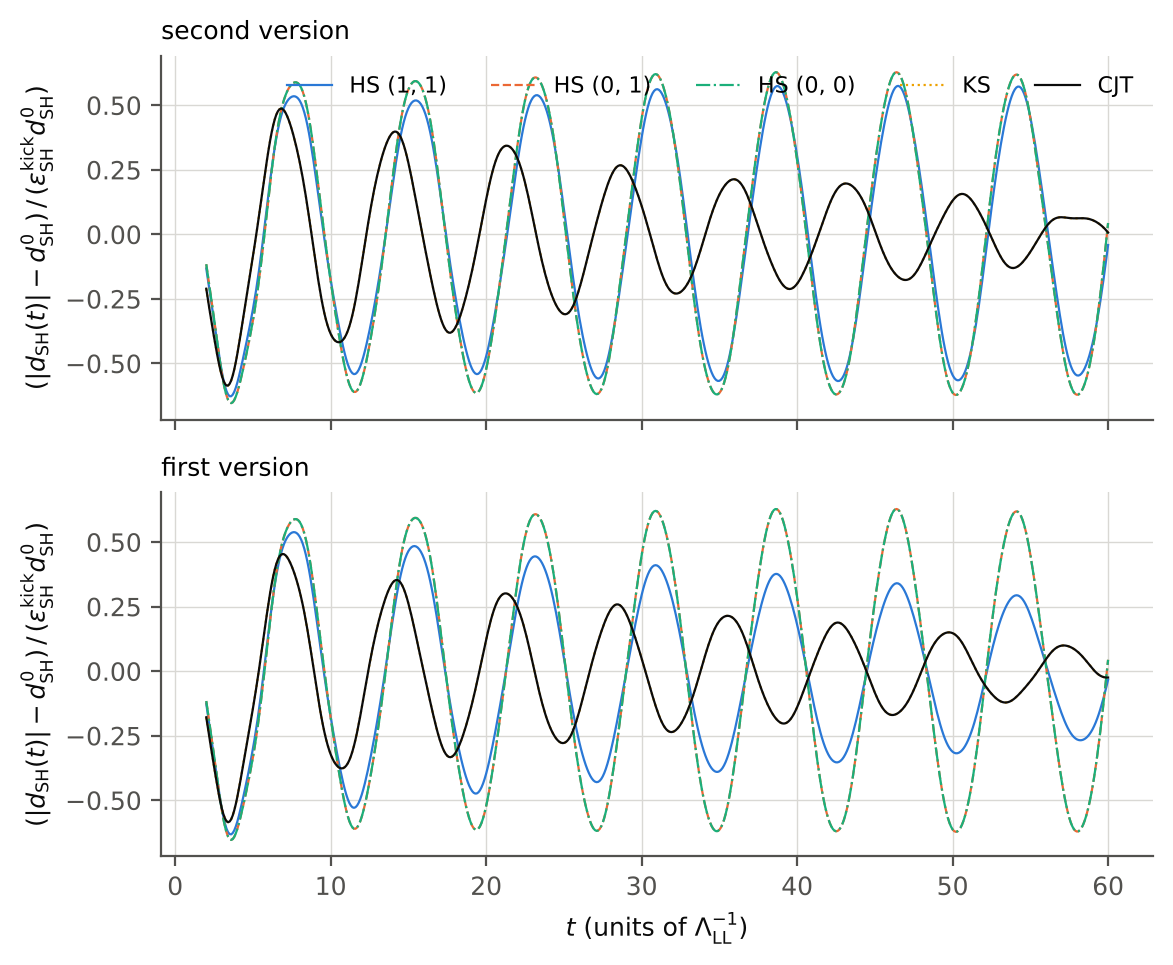
\includegraphics[width=0.92\textwidth,height=\textheight]{figures/fig_sh_dyn_amplitude.png}

\textbf{Figure 1.} The amplitude runs:
\((\lvert d_{\rm SH}(t)\rvert-d^0_{\rm SH})/(\epsilon^{\rm kick}_{\rm SH}d^0_{\rm SH})\)
for \(2\le t\le60\) in the five methods, second version (above) and
first version (below). The signals are stored every 1.0 and drawn
through their samples by band-limited interpolation. HS (0, 1) and HS
(0, 0) coincide, and so do KS and CJT.

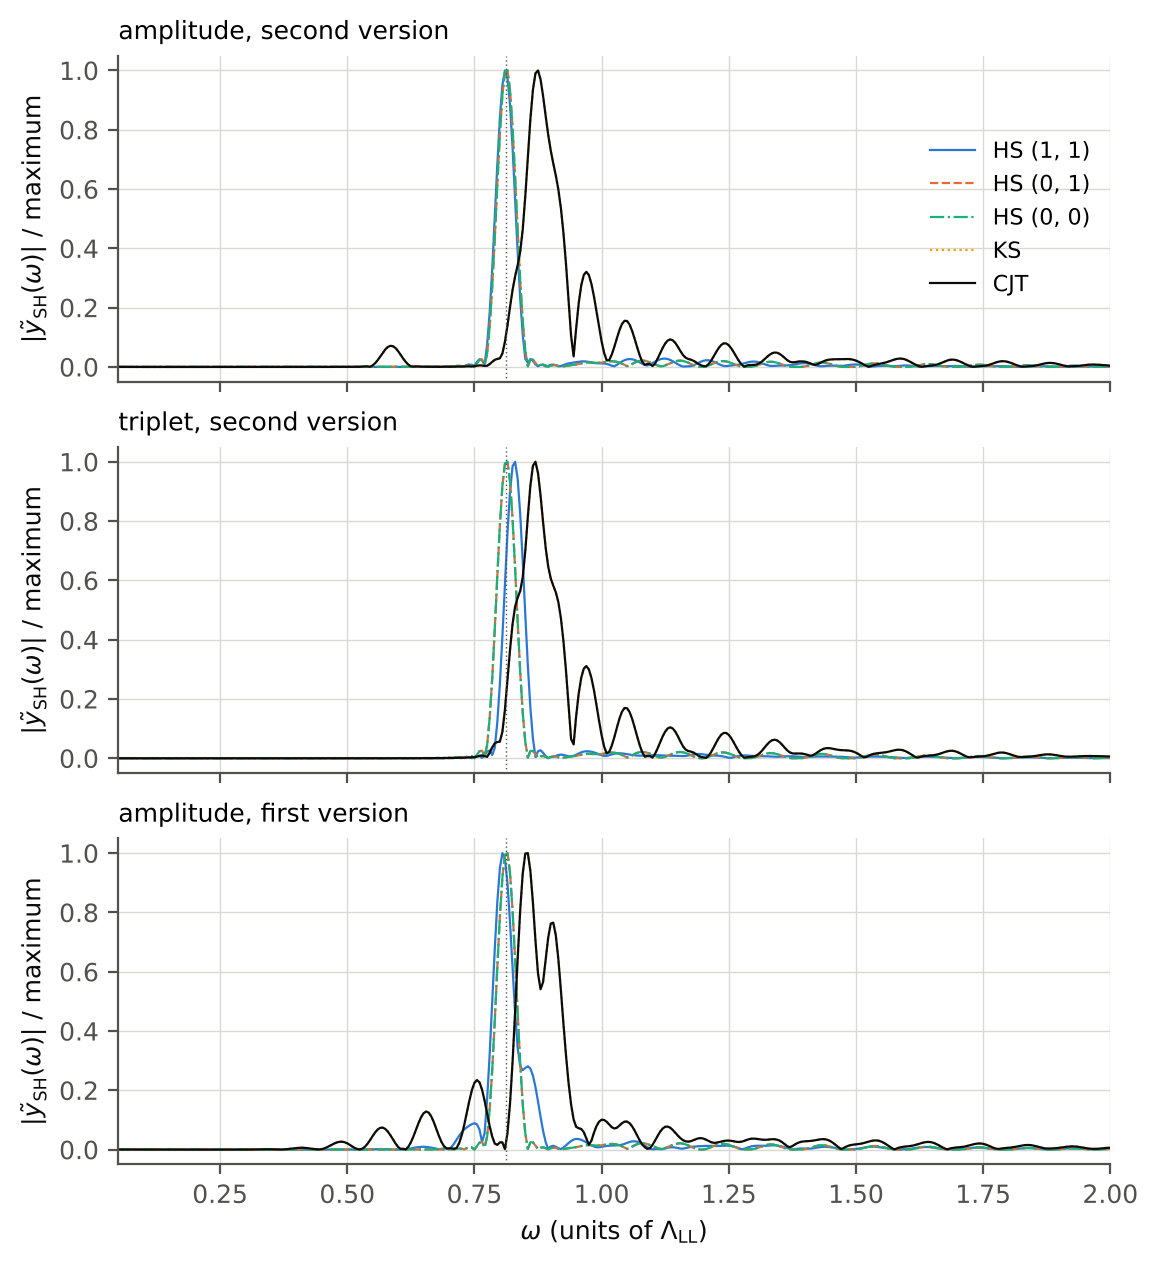
\includegraphics[width=0.92\textwidth,height=\textheight]{figures/fig_sh_dyn_spectra.png}

\textbf{Figure 2.} The spectra \(\lvert\tilde y_{\rm SH}(\omega)\rvert\)
(2.5), each divided by its largest value: the amplitude runs of the
second version (above), the triplet runs of the second version (middle)
and the amplitude runs of the first version (below). The dotted vertical
line is \(d^0_{\rm SH}\) of HS (0, 0). KS coincides with CJT.

Table 4.1. The peaks of the amplitude runs (both versions) and of the
triplet runs (second version), with \(d^0_{\rm SH}\) and twice the gap
\(E^{X,{\rm gap}}_{\rm SH}\) of stage 3, the lowest energy of two
quasi-particles. In the second version every field is paired and
\(2E^{X,{\rm gap}}_{\rm SH}\) is the energy that breaks a pair; in the
first the gap is that of the unpaired fields.

\sptkeptpenalty=10000
\begin{longtable}[]{@{}
  >{\raggedright\arraybackslash}p{(\columnwidth - 14\tabcolsep) * \real{0.1013}}
  >{\raggedright\arraybackslash}p{(\columnwidth - 14\tabcolsep) * \real{0.1392}}
  >{\raggedright\arraybackslash}p{(\columnwidth - 14\tabcolsep) * \real{0.1266}}
  >{\raggedright\arraybackslash}p{(\columnwidth - 14\tabcolsep) * \real{0.1266}}
  >{\raggedright\arraybackslash}p{(\columnwidth - 14\tabcolsep) * \real{0.1519}}
  >{\raggedright\arraybackslash}p{(\columnwidth - 14\tabcolsep) * \real{0.1013}}
  >{\raggedright\arraybackslash}p{(\columnwidth - 14\tabcolsep) * \real{0.1519}}
  >{\raggedright\arraybackslash}p{(\columnwidth - 14\tabcolsep) * \real{0.1013}}@{}}
\toprule\noalign{}
\begin{minipage}[b]{\linewidth}\raggedright
version
\end{minipage} & \begin{minipage}[b]{\linewidth}\raggedright
method
\end{minipage} & \begin{minipage}[b]{\linewidth}\raggedright
\(d^0_{\rm SH}\)
\end{minipage} & \begin{minipage}[b]{\linewidth}\raggedright
\(2E^{X,{\rm gap}}_{\rm SH}\)
\end{minipage} & \begin{minipage}[b]{\linewidth}\raggedright
\(\omega^{\rm pk}_{\rm SH}\), amplitude
\end{minipage} & \begin{minipage}[b]{\linewidth}\raggedright
\(\Gamma^{\rm pk}_{\rm SH}/\Gamma^{\rm win}_{\rm SH}\)
\end{minipage} & \begin{minipage}[b]{\linewidth}\raggedright
\(\omega^{\rm pk}_{\rm SH}\), triplet
\end{minipage} & \begin{minipage}[b]{\linewidth}\raggedright
\(\Gamma^{\rm pk}_{\rm SH}/\Gamma^{\rm win}_{\rm SH}\)
\end{minipage} \\
\midrule\noalign{}
\endhead
\bottomrule\noalign{}
\endlastfoot
second & HS (1, 1) & \(0.8328776\) & \(0.853584\) & \(0.8108707\) &
\(1\) & \(0.8285249\) & \(1\) \\*
second & HS (0, 1) & \(0.8128455\) & \(0.905935\) & \(0.8128465\) &
\(1\) & \(0.8128465\) & \(1\) \\*
second & HS (0, 0) & \(0.8128455\) & \(0.905935\) & \(0.8128465\) &
\(1\) & \(0.8128465\) & \(1\) \\*
second & KS & \(0.8907872\) & \(0.768402\) & \(0.8735459\) & \(1.8\) &
\(0.8687108\) & \(2.12\) \\*
second & CJT & \(0.8907872\) & \(0.768402\) & \(0.8735459\) & \(1.8\) &
\(0.8687108\) & \(2.12\) \\*
first & HS (1, 1) & \(0.8258096\) & \(0.340784\) & \(0.8061557\) &
\(1.04\) & -- & -- \\*
first & HS (0, 1) & \(0.8128455\) & \(0.4\) & \(0.8128466\) & \(1\) & --
& -- \\*
first & HS (0, 0) & \(0.8128455\) & \(0.4\) & \(0.8128466\) & \(1\) & --
& -- \\*
first & KS & \(0.8672856\) & \(0.222918\) & \(0.8525918\) & \(2.16\) &
-- & -- \\*
first & CJT & \(0.8672856\) & \(0.222918\) & \(0.8525918\) & \(2.16\) &
-- & -- \\
\end{longtable}

\textbf{What the table shows.}

\begin{itemize}
\tightlist
\item
  \textbf{The pairing-only methods.} In HS (0, 1) and HS (0, 0) the
  amplitude oscillates at \(d^0_{\rm SH}=0.812845546\) to
  \(2\times10^{-6}\) in both versions (check D-4a), the frequency that
  stage 4 found from the linear response and proved to be exact. The
  difference is of the order of \((\epsilon^{\rm kick}_{\rm SH})^2\),
  the size of the first correction to a linear oscillation. The peaks
  have the width of the window, \(1\) times
  \(\Gamma^{\rm win}_{\rm SH}\) (check D-4b): the mode is not damped, as
  a mode below the threshold of two quasi-particles must not be. The
  triplet oscillates at the same frequency, to \(2\times10^{-8}\) (check
  D-5): the degeneracy of the custodial singlet and triplet of stage 4.
  The Python program finds the same peaks from the stored signals
  (checks YD-3, YD-4), and the Wolfram script compares them with
  \(d^0_{\rm SH}\) to 30 digits (check WD-3).
\item
  \textbf{HS (1, 1).} The scalar and the vector terms act on the ground
  state. In the second version the amplitude mode lies at 0.810871,
  below the energy 0.853584 that breaks a pair, and its peak has the
  width of the window (1): it is bound and undamped. It is lower than
  its \(d^0_{\rm SH}=0.832878\): the closed form of the pairing-only
  methods does not hold here. The triplet lies at 0.828525, 2.2 per cent
  above the singlet, also undamped (1). In the first version the
  amplitude peak lies at 0.806156, with the width ratio 1.04.
\item
  \textbf{KS and CJT.} In the second version the spectrum of the
  amplitude peaks at 0.873546, above the energy 0.768402 that breaks a
  pair. The peak is 1.8 times wider than the window, and
  \(\lvert d_{\rm SH}(t)\rvert\) visibly decays in Figure 1: the
  amplitude mode is a resonance that decays into pairs of
  quasi-particles. The peak of the triplet lies at 0.868711 (-0.55 per
  cent from the singlet), with the width ratio 2.12. In the first
  version the amplitude peak lies at 0.852592, with the width ratio
  2.16. On a grid of 144 momenta the continuum of pairs of
  quasi-particles is a set of discrete transitions, so the decay is a
  dephasing among them, and the signal partly revives at late times; the
  width of the peak is the measure used here, not a decay rate.
\end{itemize}

The splitting of the triplet answers a question that stage 4 left open:
the degeneracy of the four massive modes of the second version is a
property of the pairing-only methods. With the scalar and the vector
terms the triplet separates from the singlet: by 2.2 per cent of its
frequency in HS (1, 1) and by -0.55 per cent in KS and CJT.

\hypertarget{the-josephson-relation-and-a-large-displacement}{%
\section{5. The Josephson relation and a large
displacement}\label{the-josephson-relation-and-a-large-displacement}}

\textbf{The Josephson relation.} A chemical potential \(\mu\) of the
particle number adds \(-\mu F^{\rm tot}_{\rm SH}\) to the Hamiltonian.
On the Nambu space \(F^{\rm tot}_{\rm SH}\) is \(\mathsf 1_{16}\) in the
particle block and \(-\mathsf 1_{16}\) in the hole block, and the
stationary state of \(\mathcal H_{\rm SH}\) evolves as
\(e^{i\mu F^{\rm tot}_{\rm SH}t}\mathcal R_{\rm SH}e^{-i\mu F^{\rm tot}_{\rm SH}t}\),
with \(F^{\rm tot}_{\rm SH}\) taken on the Nambu space: its pair block
is multiplied by \(e^{2i\mu t}\), because each pair carries the particle
number 2 (check WD-2, symbolic). The phase of \(d_{\rm SH}(t)\)
therefore turns at the rate \(2\mu=0.02\) and its length stays at
\(d^0_{\rm SH}\). The programs find the rate to \(2\times10^{-9}\) and
the length to \(2\times10^{-9}\), in HS (0, 0) and in CJT (checks D-6a,
D-6b, YD-5). This is the relation of Josephson between the chemical
potential and the frequency of the condensate; it is a check that (2.2)
treats the phase of the pair fields, the Goldstone mode of the particle
number, correctly.

\textbf{A large displacement.} Figure 3 shows the run with
\(\epsilon^{\rm kick}_{\rm SH}=0.3\) in HS (0, 0). The length of the
pair fields oscillates between 0.763 and 1.17 times \(d^0_{\rm SH}\) at
the frequency 0.778887, 0.9582 times \(d^0_{\rm SH}\). The oscillation
softens with its amplitude: the potential of the length, the Mexican hat
of stage 4, is not a parabola so far from its minimum. Both versions
give the same curve, because in HS (0, 0) each pair moves in the same
closed form.

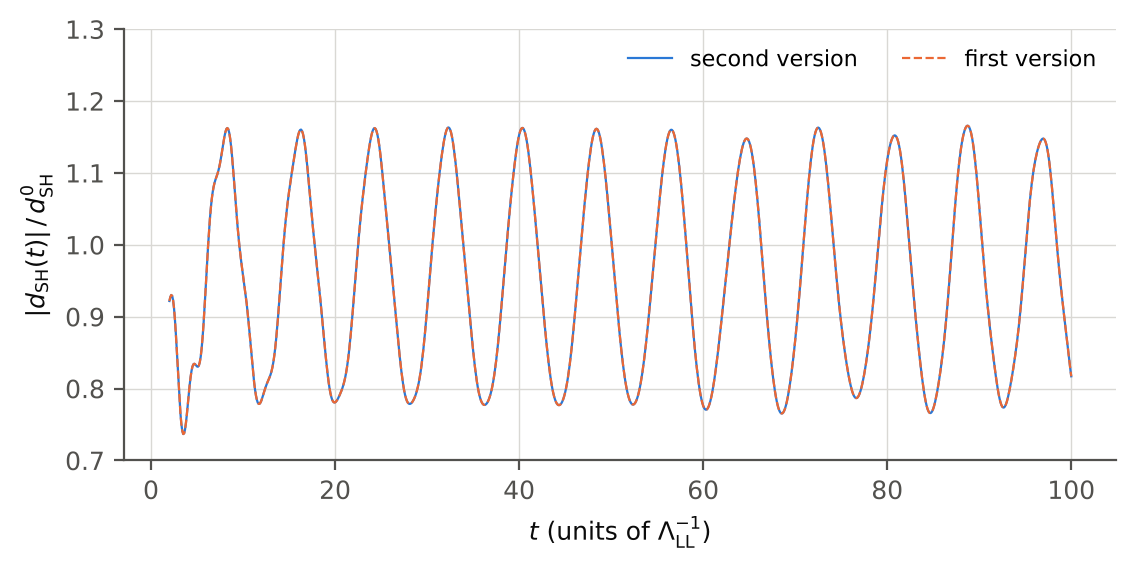
\includegraphics[width=0.92\textwidth,height=\textheight]{figures/fig_sh_dyn_large.png}

\textbf{Figure 3.} The large displacement:
\(\lvert d_{\rm SH}(t)\rvert/d^0_{\rm SH}\) for \(2\le t\le100\) in HS
(0, 0), both versions (the two curves coincide). Drawn as in Figure 1.

\hypertarget{what-the-results-mean}{%
\section{6. What the results mean}\label{what-the-results-mean}}

\begin{itemize}
\tightlist
\item
  \textbf{The time-dependent mean field is consistent with the static
  methods.} Its stationary states are the ground states of stage 3, its
  small oscillations reproduce the linear response of stage 4, it
  conserves energy, charges and orthonormality, and it obeys the
  Josephson relation.
\item
  \textbf{The amplitude mode is heavy in every method.} Where it is a
  sharp mode (HS (0, 1), HS (0, 0), HS (1, 1)) it lies near
  \(d^0_{\rm SH}\), of the order of the energy that breaks a pair. In KS
  and CJT it lies above that energy and decays. The conclusion of stage
  4 holds in all five methods: relative to the scale \(v_{\rm SH}\) the
  amplitude mode is far heavier than the Higgs boson of the Standard
  Model.
\item
  \textbf{The triplet of the second version is split.} The extra massive
  scalars of the second version are degenerate with the amplitude mode
  only in the pairing-only methods; the scalar and the vector terms
  split them, by 2.2 per cent in HS (1, 1) and by -0.55 per cent in KS
  and CJT.
\item
  \textbf{What remains.} The dynamics here is uniform in space: it
  contains the modes at zero momentum only. The gauge fields are not
  evolved, because a uniform vector potential couples through the
  current of the Dirac sea, which the sharp cutoff spoils (it gives a
  spurious current even in the normal vacuum); stage 4 found the masses
  of the gauge bosons from the time components instead. The fluctuations
  beyond the mean field are not included.
\end{itemize}

\hypertarget{the-programs-and-the-checks}{%
\section{7. The programs and the
checks}\label{the-programs-and-the-checks}}

The results were computed and checked by three programs written for this
stage:

\begin{itemize}
\tightlist
\item
  \textbf{Rust.} The program \texttt{sh\_dynamics} (crate
  \texttt{rust/shdynamics}) integrates (2.2) with CVODE through the
  crate \texttt{sfsundials} of the folder, on the static engine of
  stages 3 and 4 (the model of stage 3 included unchanged). It ran its
  12 checks and 21 runs in 2516 s on 2 threads; the longest run took 157
  s. Its verdict: ALL PASS (12 of 12).
\item
  \textbf{Python.} The program \texttt{python/sh\_dynamics.py}
  integrates (2.2) for HS (0, 0) with its own right side (numpy) and the
  same CVODE through the C interface of the folder, and analyses the
  signals of the Rust program independently: ALL PASS (7 of 7). The
  figures are drawn by \texttt{python/sh\_dynamics\_figures.py}.
\item
  \textbf{Wolfram.} The script \texttt{wolfram/source/sh\_dynamics.wls},
  run on the author's computer, derives the conservation laws, the
  Josephson relation and the width of the Hann window symbolically and
  compares the numbers of the Rust program with them: ALL PASS (5 of 5).
\end{itemize}

The reports are \texttt{data/hck\_sh\_dynamics\_checks.txt},
\texttt{data/hck\_sh\_dynamics\_checks\_python.txt} and
\texttt{data/hck\_sh\_dynamics\_checks\_wolfram.txt}. The data are:

\begin{itemize}
\tightlist
\item
  \texttt{data/sh\_dyn\_runs.csv}: for each run the peak of its
  spectrum, its width, the conservation laws and the work of CVODE;
\item
  \texttt{data/sh\_dyn\_signals.csv}: \(d_{\rm SH}(t)\),
  \(d^{\rm trip}_{\rm SH}(t)\) and the energy per volume of every run,
  every 1.0;
\item
  \texttt{data/sh\_dyn\_spectra.csv}:
  \(\lvert\tilde y_{\rm SH}(\omega)\rvert\) of the amplitude, triplet
  and large runs for \(0.05\le\omega\le2.5\);
\item
  \texttt{data/sh\_dyn\_values.csv}: the settings and the ground states.
\end{itemize}

The tables and numbers of this document are written from them by
\texttt{code/scripts/write\_sh\_dynamics\_fragments.py}. The commands,
from the folder \texttt{Revision\_SM\_Higgs}:

\begin{Shaded}
\begin{Highlighting}[]
\CommentTok{\# the Rust program (after sh\_superfluid and sh\_higgs, whose data it reads)}
\KeywordTok{(}\BuiltInTok{cd}\NormalTok{ rust }\KeywordTok{\&\&} \ExtensionTok{cargo}\NormalTok{ build }\AttributeTok{{-}{-}release} \KeywordTok{\&\&} \ExtensionTok{./target/release/sh\_dynamics}\KeywordTok{)}
\CommentTok{\# the Python program and the figures (after the Rust program)}
\KeywordTok{(}\BuiltInTok{cd}\NormalTok{ python }\KeywordTok{\&\&} \ExtensionTok{python3}\NormalTok{ sh\_dynamics.py}\KeywordTok{)}
\ExtensionTok{python3}\NormalTok{ python/sh\_dynamics\_figures.py}
\CommentTok{\# the Wolfram script (on a computer with Wolfram)}
\ExtensionTok{wolframscript} \AttributeTok{{-}file}\NormalTok{ wolfram/source/sh\_dynamics.wls data/sh\_dyn\_runs.csv data/sh\_dyn\_signals.csv }\DataTypeTok{\textbackslash{}}
\NormalTok{    data/hck\_sh\_dynamics\_checks\_wolfram.txt}
\CommentTok{\# the tables and numbers of this document}
\ExtensionTok{python3}\NormalTok{ code/scripts/write\_sh\_dynamics\_fragments.py}
\end{Highlighting}
\end{Shaded}

The Rust program \texttt{sh\_dynamics}:

\begin{longtable}[]{@{}
  >{\raggedright\arraybackslash}p{(\columnwidth - 8\tabcolsep) * \real{0.0947}}
  >{\raggedright\arraybackslash}p{(\columnwidth - 8\tabcolsep) * \real{0.0632}}
  >{\raggedright\arraybackslash}p{(\columnwidth - 8\tabcolsep) * \real{0.1053}}
  >{\raggedright\arraybackslash}p{(\columnwidth - 8\tabcolsep) * \real{0.0947}}
  >{\raggedright\arraybackslash}p{(\columnwidth - 8\tabcolsep) * \real{0.6421}}@{}}
\toprule\noalign{}
\begin{minipage}[b]{\linewidth}\raggedright
check
\end{minipage} & \begin{minipage}[b]{\linewidth}\raggedright
result
\end{minipage} & \begin{minipage}[b]{\linewidth}\raggedright
deviation
\end{minipage} & \begin{minipage}[b]{\linewidth}\raggedright
tolerance
\end{minipage} & \begin{minipage}[b]{\linewidth}\raggedright
statement
\end{minipage} \\
\midrule\noalign{}
\endhead
\bottomrule\noalign{}
\endlastfoot
D-1 & PASS & 2.320e-10 & 1.0e-8 & the integrator (CVODE, Adams-Moulton,
rtol 1e-12, atol 1e-14): y'\,' = -y from (1, 0) over 0 \textless= t
\textless= 100 against (cos t, -sin t) (largest absolute deviation at
the 1001 output times) \\
D-2 & PASS & 3.736e-9 & 1.0e-7 & the ground state stays at rest: the
largest /d(t) - d\_0/ / d\_0 over 0 \textless= t \textless= 100, second
version, HS (0, 0) and CJT \\
D-3a & PASS & 1.097e-6 & 1.0e-5 & the energy per volume is conserved in
every run (largest /E(t) - E(0)/ relative to the largest /E(t)/ of the
run; the largest in amplitude\_first\_HS0\_1); the energy per volume is
the difference of its kinetic and interaction parts, each about ten
times larger, and its drift follows the loss of orthonormality of D-3c
that the integration error causes (the exact flow conserves it: check
WD-1) \\
D-3b & PASS & 6.115e-10 & 1.0e-9 & the charge densities of the
symmetries are conserved in every run (all eight generators in the
second version; T\^{}1, T\^{}2, T\^{}3, T\^{}3\_R, R, F\_tot in the
first; largest absolute change) \\
D-3c & PASS & 1.991e-8 & 1.0e-7 & the evolution is unitary: the largest
/V(q)\^{}dag V(q) - 1/ over the nodes at the end of every run \\
D-4a & PASS & 1.239e-6 & 1.0e-4 & the amplitude mode in the time domain:
the peak of the spectrum of /d(t)/ after the kick eps = 1e-3 lies at
d\_0, the frequency of the linear response of stage 4 (relative), HS (0,
1) and HS (0, 0), both versions {[}second HS (0, 1): peak 0.81284655
against d\_0 = 0.81284555, width ratio 1.0000; second HS (0, 0): peak
0.81284655 against d\_0 = 0.81284555, width ratio 1.0000; first HS (0,
1): peak 0.81284655 against d\_0 = 0.81284555, width ratio 1.0000; first
HS (0, 0): peak 0.81284655 against d\_0 = 0.81284555, width ratio
1.0000{]} \\
D-4b & PASS & 5.048e-6 & 2.0e-2 & the amplitude mode is undamped over
the run: the half width of its peak equals that of a pure cosine sampled
in the same way, the width of the window (largest ratio minus 1), HS (0,
1) and HS (0, 0), both versions \\
D-5 & PASS & 1.975e-8 & 1.0e-4 & second version, HS (0, 1) and HS (0,
0): the neutral member of the custodial triplet oscillates at the
frequency of the amplitude mode (relative difference of the peaks), the
degeneracy of stage 4 \\
D-6a & PASS & 1.045e-9 & 1.0e-6 & the Josephson relation: with H - mu
F\_tot (mu = 0.01) the phase of d(t) turns at the rate 2 mu (relative
difference of the modulus of the fitted rate; each pair carries the
particle number 2), second version, HS (0, 0) and CJT {[}second HS (0,
0): rate 0.019999999979 (2 mu = 0.02), largest / /d/ - d\_0 / / d\_0
1.5e-9; second CJT: rate 0.020000000013 (2 mu = 0.02), largest / /d/ -
d\_0 / / d\_0 2.9e-10{]} \\
D-6b & PASS & 1.481e-9 & 1.0e-7 & in the same runs /d(t)/ stays at d\_0
(largest relative deviation) \\
D-7 & PASS & 4.573e-8 & 1.0e-6 & KS and CJT give the same dynamics: the
largest /d\_KS(t) - d\_CJT(t)/ / d\_0 in the amplitude runs of both
versions and of d\_trip(t) in the triplet runs \\
D-8 & PASS & -- & -- & in the methods with normal self-energies (HS (1,
1), KS, CJT) the spectra of the amplitude runs (both versions) and of
the triplet runs (second version) have a peak; reported with twice the
gap of stage 3 and d\_0 (second HS (1, 1): amplitude peak 0.810871 (2
E\_gap 0.853584, d\_0 0.832878), width ratio 1.000, triplet peak
0.828525, width ratio 1.001; second KS: amplitude peak 0.873546 (2
E\_gap 0.768402, d\_0 0.890787), width ratio 1.800, triplet peak
0.868711, width ratio 2.120; second CJT: amplitude peak 0.873546 (2
E\_gap 0.768402, d\_0 0.890787), width ratio 1.800, triplet peak
0.868711, width ratio 2.120; first HS (1, 1): amplitude peak 0.806156 (2
E\_gap 0.340784, d\_0 0.825810), width ratio 1.038; first KS: amplitude
peak 0.852592 (2 E\_gap 0.222918, d\_0 0.867286), width ratio 2.159;
first CJT: amplitude peak 0.852592 (2 E\_gap 0.222918, d\_0 0.867286),
width ratio 2.159) \\
\end{longtable}

The Python program \texttt{python/sh\_dynamics.py}:

\sptkeptpenalty=10000
\begin{longtable}[]{@{}
  >{\raggedright\arraybackslash}p{(\columnwidth - 8\tabcolsep) * \real{0.0947}}
  >{\raggedright\arraybackslash}p{(\columnwidth - 8\tabcolsep) * \real{0.0632}}
  >{\raggedright\arraybackslash}p{(\columnwidth - 8\tabcolsep) * \real{0.1053}}
  >{\raggedright\arraybackslash}p{(\columnwidth - 8\tabcolsep) * \real{0.0947}}
  >{\raggedright\arraybackslash}p{(\columnwidth - 8\tabcolsep) * \real{0.6421}}@{}}
\toprule\noalign{}
\begin{minipage}[b]{\linewidth}\raggedright
check
\end{minipage} & \begin{minipage}[b]{\linewidth}\raggedright
result
\end{minipage} & \begin{minipage}[b]{\linewidth}\raggedright
deviation
\end{minipage} & \begin{minipage}[b]{\linewidth}\raggedright
tolerance
\end{minipage} & \begin{minipage}[b]{\linewidth}\raggedright
statement
\end{minipage} \\
\midrule\noalign{}
\endhead
\bottomrule\noalign{}
\endlastfoot
YD-1 & PASS & 3.733e-10 & 1.0e-08 & HS (0, 0), both versions: the kick
eps = 1e-3 along the vacuum direction integrated here (numpy and CVODE,
rtol 1e-12, atol 1e-14) to t = 100; d(t) against the Rust program every
1.0 (largest /difference/ / d\_0) {[}second: largest /d\_Python -
d\_Rust/ / d\_0 = 4.32e-11 (CVODE: 2049 steps, 4090 evaluations of the
right side, 3 rejected steps, 4087 fixed-point iterations (0 convergence
failures), last order 7, last step 4.9437e-02); first: largest
/d\_Python - d\_Rust/ / d\_0 = 3.73e-10 (CVODE: 1899 steps, 3790
evaluations of the right side, 3 rejected steps, 3787 fixed-point
iterations (0 convergence failures), last order 7, last step
5.3391e-02){]} \\*
YD-2a & PASS & 3.611e-07 & 1.0e-05 & in the same runs the energy per
volume is conserved (largest /E(t) - E(0)/ relative to the largest /E/;
the energy per volume is the difference of its kinetic and interaction
parts, each about ten times larger, and its drift follows the loss of
orthonormality that the integration error causes) \\*
YD-2b & PASS & 5.922e-09 & 1.0e-07 & in the same runs the vectors stay
orthonormal (largest /V\^{}dag V - 1/ at t = 100) \\*
YD-3 & PASS & 1.241e-06 & 1.0e-04 & the peaks of the spectra of /d(t)/
of the amplitude runs of HS (0, 1) and HS (0, 0) of the Rust program,
computed here from the samples every 1.0, lie at d\_0 = 0.8128455463 of
the closed-form gap equation (relative) {[}second HS0\_1: 0.81284655;
second HS0\_0: 0.81284655; first HS0\_1: 0.81284655; first HS0\_0:
0.81284655{]} \\*
YD-4 & PASS & 7.036e-09 & 1.0e-04 & the peaks of all 17 amplitude,
triplet and large runs computed here (samples every 1.0) agree with
those of the Rust program (samples every 0.2; data/sh\_dyn\_runs.csv;
relative) \\*
YD-5 & PASS & 1.045e-09 & 1.0e-06 & the Josephson runs of the Rust
program: the unwrapped phase of d(t) grows linearly at the rate 2 mu =
0.02 (relative difference of the modulus of the fitted rate)
{[}josephson\_second\_HS0\_0: rate 0.019999999979;
josephson\_second\_CJT: rate 0.020000000013{]} \\*
YD-6 & PASS & 6.022e-09 & 1.0e-07 & HS (0, 0): the reduced model of
Anderson pseudospins, one at +eps\_k and one at -eps\_k = -(k\^{}2 +
m\^{}2)\^{}(1/2) for each of the 24 radial nodes (each with half the
weight of the node), with the gap parameter d / 2, reproduces d(t) of
the Rust program for 0 \textless= t \textless= 100 after the kicks eps =
1e-3 and 0.3, both versions (largest /difference/ / d\_0; d\_0 of the
reduced model is 0.812845546320) {[}amplitude\_second\_HS0\_0: 3.7e-09;
large\_second\_HS0\_0: 1.1e-09; amplitude\_first\_HS0\_0: 6.0e-09;
large\_first\_HS0\_0: 1.3e-09{]} \\
\end{longtable}

The Wolfram script \texttt{wolfram/source/sh\_dynamics.wls}:

\sptkeptpenalty=10000
\begin{longtable}[]{@{}
  >{\raggedright\arraybackslash}p{(\columnwidth - 8\tabcolsep) * \real{0.0947}}
  >{\raggedright\arraybackslash}p{(\columnwidth - 8\tabcolsep) * \real{0.0632}}
  >{\raggedright\arraybackslash}p{(\columnwidth - 8\tabcolsep) * \real{0.1053}}
  >{\raggedright\arraybackslash}p{(\columnwidth - 8\tabcolsep) * \real{0.0947}}
  >{\raggedright\arraybackslash}p{(\columnwidth - 8\tabcolsep) * \real{0.6421}}@{}}
\toprule\noalign{}
\begin{minipage}[b]{\linewidth}\raggedright
check
\end{minipage} & \begin{minipage}[b]{\linewidth}\raggedright
result
\end{minipage} & \begin{minipage}[b]{\linewidth}\raggedright
deviation
\end{minipage} & \begin{minipage}[b]{\linewidth}\raggedright
tolerance
\end{minipage} & \begin{minipage}[b]{\linewidth}\raggedright
statement
\end{minipage} \\
\midrule\noalign{}
\endhead
\bottomrule\noalign{}
\endlastfoot
WD-1 & PASS & -- & -- & the time-dependent mean field i dR/dt = {[}H,
R{]} conserves tr(H R) when H is the derivative of the energy (d tr(H
R)/dt = -i tr(H {[}H, R{]}) = 0), keeps R Hermitian, and keeps a
projector a projector (symbolic, 3 x 3 Hermitian matrices with symbolic
entries; the projector of rank 1 along the first axis) (energy True,
hermiticity True, projector True) \\*
WD-2 & PASS & -- & -- & the Josephson relation: exp(i mu F t) R\_0
exp(-i mu F t) solves i dR/dt = {[}H - mu F, R{]} for a stationary R\_0
and multiplies the pair block by exp(2 i mu t) (symbolic); the phases of
d(t) of the Josephson runs of the Rust program grow at the rate 2 mu =
0.02 (straight-line fit in exact arithmetic on the numbers of the file;
relative) (rates josephson\_second\_HS0\_0 0.0199999999791,
josephson\_second\_CJT 0.0200000000125; deviation
1.0453166110480083e-9) \\*
WD-3 & PASS & -- & -- & the peaks of the amplitude runs of HS (0, 1) and
HS (0, 0) of the Rust program (both versions) lie at d\_0 =
0.81284554632043386736 of the gap equation (relative) (deviation
1.2e-6) \\*
WD-4 & PASS & -- & -- & the Hann window: its normalized transform has
the modulus /sin(x pi) / (x pi (1 - x\^{}2))/ at the offset x 2 pi / T
(the squared modulus of the exact integral equals that of the closed
form at nine rational offsets, exactly) and the value 1/2 at x = 1
(limit), so that the half width at half maximum of a pure cosine is 2 pi
/ T = 0.020943951 for the runs of length 300; the widths of the sampled
cosines of the Rust program against it (relative) (form True, half True,
deviation 5.e-7) \\*
WD-5 & PASS & -- & -- & HS (0, 0): the reduced model of 48 Anderson
pseudospins (one at +eps\_k and one at -eps\_k for each of the 24 radial
nodes, eps\_k = (k\^{}2 + m\^{}2)\^{}(1/2)), integrated here by NDSolve
with the method IDA, gives d\_0 = 2 Delta\_0 = 0.812845546320434 from
its gap equation and, after the kick 1e-3, the d(t) of the Rust program
for 0 \textless= t \textless= 50 (largest /difference/ / d\_0, at the 51
stored times) (d\_0 against the gap equation of WD-3 6.e-22; deviation
1.7485437131808761e-9) \\
\end{longtable}

\hypertarget{the-symbols-of-this-document}{%
\section{8. The symbols of this
document}\label{the-symbols-of-this-document}}

\begin{longtable}[]{@{}
  >{\raggedright\arraybackslash}p{(\columnwidth - 2\tabcolsep) * \real{0.5000}}
  >{\raggedright\arraybackslash}p{(\columnwidth - 2\tabcolsep) * \real{0.5000}}@{}}
\toprule\noalign{}
\begin{minipage}[b]{\linewidth}\raggedright
symbol
\end{minipage} & \begin{minipage}[b]{\linewidth}\raggedright
meaning
\end{minipage} \\
\midrule\noalign{}
\endhead
\bottomrule\noalign{}
\endlastfoot
\(\Psi_{\rm LL}\); \(\chi_{\rm SH}\), \(\chi'_{\rm SH}\);
\(\Psi_{\rm SH}\) & the isodoublet of Dirac fields (eight components,
component \(2d+s\)), the two singlet Dirac fields (four components
each), and the three as one field of sixteen components \\
\(m_{\rm LL}\), \(m^\chi_{\rm SH}\), \(m^{\chi'}_{\rm SH}\) & the masses
of the three fields (all \(0.2\,\Lambda_{\rm LL}\)) \\
\(\Lambda_{\rm LL}\) & the momentum cutoff, the unit of the
computation \\
\(SL(2,\mathbb C)\), \(SU(2)_L\), \(U(1)_Y\) & the Lorentz group of the
spinors and the electroweak gauge group \\
\(T^{a,{\rm SM}}\), \(\tau^a\); \(Y^{\rm SM}\), \(Q^{\rm SM}\) & the
generators of \(SU(2)_L\) and the Pauli matrices; the hypercharge and
the electric charge \\
\(F^{\rm tot}_{\rm SH}\), \(R_{\rm SH}\) & the particle number and the
relative number \\
\(SU(2)_{\rm R}\), \(T^{a,{\rm R}}_{\rm SH}\); \(SU(2)_{\rm V}\) & the
custodial group, which acts on \((\chi_{\rm SH},\chi'_{\rm SH})\) as on
a doublet, and its generators; the diagonal subgroup of
\(SU(2)_L\times SU(2)_{\rm R}\) \\
\(\gamma^p_{\rm LL}\), \(\beta_{\rm LL}\), \(\alpha^j_{\rm LL}\),
\(\gamma^{\rm ch}_{\rm LL}\), \(C_{\rm LL}\); \(\sigma^{\rm LL}_j\) &
the Dirac matrices of the chiral basis, the chirality matrix, the
charge-conjugation matrix; the Pauli matrices on a Weyl spinor \\
\(\vec q_{\rm LL}\), \(q^j_{\rm LL}\) & a momentum and its components \\
\(\mathbf e^{\rm u}_{\rm SH}\), \(\mathbf e^{\rm d}_{\rm SH}\)
(\(\mathbf e^s_{\rm SH}\)) & the isospin columns \((1,0)^T\) and
\((0,1)^T\) \\
\(\Pi^s_{\rm SH}\), \(\Pi'^s_{\rm SH}\); \(\mathsf K^s_{\rm SH}\),
\(\mathsf K'^s_{\rm SH}\) & the pair operators (1.1) and their
\(16\times16\) pair matrices \\
\(\Phi_{\rm SH}\), \(\Phi'_{\rm SH}\) & the two pair fields \\
\(\mathcal H_{\rm SH}\), \(\mathsf h_{\rm SH}(\vec q_{\rm LL})\) & the
Hamiltonian density (1.2) and the free Hamiltonian of the sixteen
components on a plane wave \\
\(\bar\Psi_{\rm LL}\); \({:}\ {:}\) & the Dirac adjoint; the normal
ordering with respect to the normal vacuum \\
\(G^{\rm S}_{\rm SF}\), \(G^{\rm V}_{\rm SF}\), \(G_{\rm SH}\);
\(V^{(1)}_{\rm SH}\) & the couplings of the scalar, the vector and the
pairing terms; the potential with \(G^{\rm S}_{\rm SF}=-8\),
\(G^{\rm V}_{\rm SF}=0.8\), \(G_{\rm SH}=100.8\) \\
\(\mathsf N_{\rm SH}\), \(\mathsf P_{\rm SH}\);
\(\mathsf H_{\rm SH}(\vec q_{\rm LL})\) & the normal and the pair
self-energies of a uniform state; its BdG matrix (1.3) \\
\(\mathsf N^0_{\rm SH}\), \(\mathsf P^0_{\rm SH}\) & the self-energies
of the ground state \\
\(\varrho_{\rm SH}\), \(\kappa_{\rm SH}\) & the local normal matrix,
measured from the normal vacuum, and the local pair matrix \\
\(\mathcal E^X_{\rm SH}\) & the energy per volume of a uniform state in
method \(X\), measured from the normal vacuum \\
\(X\); \(s^{\rm HS,S}_{\rm SF}\), \(s^{\rm HS,V}_{\rm SF}\) & a method
(HS (1, 1), HS (0, 1), HS (0, 0), KS or CJT); the HS parameters \\
\(\mathsf P^{\rm vac}_{\rm SH}\); \(d_{\rm SH}\), \(d^0_{\rm SH}\) & the
direction (1.4) of the vacuum in the pair self-energy; the coefficient
(2.4) of a pair self-energy along it, and its value in the ground
state \\
\(\mathsf P^{\rm trip}_{\rm SH}\), \(d^{\rm trip}_{\rm SH}\) & the
direction (2.3) of the neutral member of the custodial triplet; the
coefficient (2.4) along it \\
\(\mathsf O_{\rm SH}(\vec q_{\rm LL},t)\) & the \(32\times16\) matrix of
the occupied quasi-particle vectors of a uniform state \\
\(\mathcal R_{\rm SH}(\vec q_{\rm LL},t)\) & the generalized density
(2.1) of the sixteen components \\
\(t\); \(t^{\rm end}_{\rm SH}\); \(t_i\), \(\Delta t\) & the time; the
length of a run; the output times and their spacing \\
\(w(\vec q)\) & the weight of the momentum \(\vec q\) in the sums over
the grid \\
\(\epsilon^{\rm kick}_{\rm SH}\) & the displacement of a run, relative
to \(d^0_{\rm SH}\) \\
\(\mu\) & the chemical potential of the particle number in the Josephson
runs \\
\(E^{X,{\rm gap}}_{\rm SH}\) & the gap of a ground state of stage 3: the
lowest energy of one quasi-particle \\
\(\mathbf n^\pm_{\rm SH}(q_i,t)\), \(n^{\pm,x}_{{\rm SH},i}\),
\(n^{\pm,y}_{{\rm SH},i}\); \(\mathbf b^\pm_{\rm SH}\);
\(\Delta_{\rm SH}(t)\) & the pseudospins (2.6) of the particles and of
the antiparticles at the radial node \(q_i\), and their components;
their fields; the gap parameter (2.7) \\
\(q_i\), \(w_i\); \(E_i\); \(\varepsilon_{\rm LL}\) & a radial node of
the grid and its weight times \(q_i^2/(2\pi^2)\); the energy of a
quasi-particle at it; the free energy
\((q_{\rm LL}^2+m_{\rm LL}^2)^{1/2}\) \\
\(y_{\rm SH}(t)\), \(\tilde y_{\rm SH}(\omega)\);
\(h^{\rm Hann}_{\rm SH}(t)\) & the signal of a run and its transform
(2.5); the Hann window \\
\(\omega\); \(\omega^{\rm pk}_{\rm SH}\), \(\Gamma^{\rm pk}_{\rm SH}\),
\(\Gamma^{\rm win}_{\rm SH}\) & a frequency; the frequency and the half
width at half maximum of the largest peak of a spectrum, and the half
width of the window \\
\(v_{\rm SH}\) & the scale of the breaking of \(SU(2)_L\times U(1)_Y\)
by the superfluid \\
\(a\), \(d\), \(s\), \(j\), \(p\), \(i\), \(x\) & indices: generators,
the Dirac index, the isospin index, the space coordinates, the spacetime
coordinates, the output times; an offset in units of
\(2\pi/t^{\rm end}_{\rm SH}\) \\
\(\mathsf 1_2\), \(\mathsf 1_4\), \(\mathsf 1_{16}\), \(\mathsf 1\);
\({}^T\), \({}^\dagger\), \(\otimes\), \(\mathrm{tr}\), \(\mathrm{Re}\)
& unit matrices; the transpose, the Hermitian conjugate, the Kronecker
product, the trace, the real part \\
\end{longtable}

\end{document}
